\documentclass[tikz, tcolorbox]{summary}
%=================================================================
\title{Summary}
\headtitle{PROBABILISTIC AI -- SUMMARY}
\author{PETER BREUER}

\usepackage[cmbright]{sfmath}

\usepackage{algpseudocode} % pseudocode

\begin{document}

	% restart page counter
	\setcounter{page}{1}
	% reactivate header and footer
	\pagestyle{plain}

	\begin{multicols*}{3}
		\LARGE \textbf{\colorbox{black}{\textcolor{white}{PROBABILISTIC AI}}} \\
		\normalsize 
        %\textbf{\colorbox{color2}{\textcolor{white}{\url{URL}}}} \\
        \textbf{\colorbox{color2}{\textcolor{white}{\href{mailto:pbreuer@ethz.ch}{PBREUER}}}}
        \blue{Rev: \today}
        \normalsize
        \raggedcolumns
        
		\section{PROBABILITY}

\begin{yellowbox}{\textbf{NOMENCLATURE}}
    \begin{tabularx}{\columnwidth}{ll}
        $\Omega$ & Sample space\\
        \addlinespace[2pt]
        $\mathcal{F}\subseteq 2^\Omega$ & Event space \\
        \addlinespace[2pt]
        $A,B,C$ & Events\\
        \addlinespace[2pt]
        $X,Y,Z$ & Random variables (RVs)\\
        \addlinespace[2pt]
        $x,y,z$ & States of RVs $X,Y,Z$, respectively\\
        \addlinespace[2pt]
        $P(A):\mathcal{F}\to[0,1]$ & Probability that event $A\in\mathcal{F}$ happens\\
        \addlinespace[2pt]
        $P(X=x)$ & Probability of RV $X$ assuming state $x$\\
        \addlinespace[2pt]
        $p_X(x)=:p(x)$ & \makecell[l]{Probability mass function (PMF)\\ for discrete RV $X$}\\
        \addlinespace[2pt]
        $f_X(x)=:f(x)$ & \makecell[l]{Probability density function (PDF)\\ for continuous RV $X$}\\
        \addlinespace[2pt]
        $F_X(x)=:F(x)$ & \makecell[l]{Cumulative distribution function (CDF)}\\
        \addlinespace[2pt]
        $\mathbb{E}_X[X]=:\mathbb{E}[X]$ & Expectation of $X$\\
        \addlinespace[2pt]
        $\mathrm{Var}[X]$ & Variance of $X$
    \end{tabularx}
\end{yellowbox}

\begin{whitebox}{\textbf{PROBABILITY SPACE AXIOMS}}
    \begin{itemize}
        \item Normalization
        \begin{align*}
            P(\Omega)=1
        \end{align*}
        \item Non-negativity
        \begin{align*}
            P(A)\geq0\ \forall A\in\mathcal{F}
        \end{align*}
        \item $\sigma$-additivity
        \begin{align*}
            \forall A_1,\hdots, A_n,\hdots\in\mathcal{F}\text{ disjoint:}\\
            \left(\bigcup_{i=1}^{\infty} A_i\right)=\sum_{i=1}^{\infty} P\left(A_i\right)
        \end{align*}
    \end{itemize}
\end{whitebox}

\begin{whitebox}{\textbf{DISTRIBUTIONS OF RANDOM VARIABLES}}
    \begin{itemize}
        \item Cumulative distribution function (CDF)
        \begin{align*}
            &F_X(x)=P(X\leq x)\\
            &P(X\in(x_1,x_2])=F_X(x_2)-F_X(x_1)
        \end{align*}
        \item Probability mass function (PMF) for discrete RVs
        \begin{align*}
            P(X=x)=p_X(x)
        \end{align*}
        \item Probability density function (PDF) for continuous RVs
        \begin{align*}
            P(X\in[x_1,x_2])=\int_{x_1}^{x_1}f_X(x)\ dx
        \end{align*}
    \end{itemize}
\end{whitebox}

\begin{whitebox}{\textbf{EXPECTATION}}
    \begin{itemize}
        \item Continuous RV $x$
        \begin{align*}
            \mathbb{E}[X]:=\mathbb{E}_{x\sim f(x)}[X]=\int_{-\infty}^{\infty}x\ f(x)\ dx\\
        \end{align*}
        \begin{itemize}
            \item Expectation of a function $g(x)$
            \begin{align*}
                \mathbb{E}_{x\sim f(x)}[g(x)]=\int_{-\infty}^{\infty}g(x)\ f(x)\ dx
            \end{align*}
        \end{itemize}
        \item Discrete RV $x$
        \begin{align*}
            \mathbb{E}[X]:=\mathbb{E}_{x\sim p(x)}[X]=\sum_i x_i\ p(x_i)
        \end{align*}
        \begin{itemize}
            \item Expectation of a function $g(x)$
            \begin{align*}
                \mathbb{E}_{x\sim p(x)}[g(x)]=\sum_i g(x_i)\ p(x_i)
            \end{align*}
        \end{itemize}
        \item Property
        \begin{align*}
            \mathbb{E}[aX+Y+b]=a\mathbb{E}[X]+\mathbb{E}[Y]+b\\
        \end{align*}
    \end{itemize}
\end{whitebox}

\begin{whitebox}{\textbf{VARIANCE}}
    \begin{align*}
        &\mathrm{Var}[X]:=\mathbb{E}[(X-\mathbb{E}[X])^2]=\mathbb{E}[X^2]-\mathbb{E}[X]^2\\
        &\mathrm{Var}[aX+bY+c]=a^2\mathrm{Var}[X]+b^2\mathrm{Var}[Y]+2ab\mathrm{Cov}[X,Y]\\
        &\mathrm{Var}[aX-bY+c]=a^2\mathrm{Var}[X]+b^2\mathrm{Var}[Y]-2ab\mathrm{Cov}[X,Y]\\
    \end{align*}
\end{whitebox}

\begin{whitebox}{\textbf{INDEPENDENCE}}
    \begin{itemize}
        \item Independent discrete RVs $X,Y,Z$
        \mathbox{
            P(X,Y,Z)=P(X)\cdot P(Y)\cdot P(Z)
        }
        \begin{align*}
            \Longleftrightarrow P(X|Y)=P(X),\quad P(Y)>0
        \end{align*}
        \item Independent continuous RVs
        \begin{align*}
            &F_{X,Y}(x,y)=F_X(x)F_Y(y)\\
            &f_{X,Y}(x,y)=f_X(x)f_Y(y)
        \end{align*}
        \item Discrete RVs $X,Y$ conditionally independent given $Z$
        \mathbox{
        P(X,Y| Z)=P(X| Z)\cdot P(Y| Z)
        }
        \begin{align*}
            \Longleftrightarrow P(X| Y,Z)=P(X| Z),\quad P(Y| Z)>0
        \end{align*}
        \begin{itemize}
            \item Given information provided by $Z$, $Y$ doesn't provide additional information on $X$
            \item Notation for sets of RVs $\bm{X,Y,Z}$
            \begin{align*}
                \bm{X}\perp \bm{Y}|\bm{Z}
            \end{align*}

        \end{itemize}
    \end{itemize}
\end{whitebox}

\begin{whitebox}{\textbf{RULES}}
    \begin{itemize}
        \item Conditional probability
      \mathbox{
          P(A| B)=\frac{P(A,B)}{P(B)},\quad P(B)\neq0
      }
      \item Product rule
      \begin{align*}
          P(X_{1:n})=P(X_1)\cdot P(X_2| X_1)\cdot P(X_3| X_{1:2})\cdot\hdots\cdot P(X_n| X_{1:n-1})
      \end{align*}
       \item Sum rule (marginalization)
        \mathbox{
            P(X_{1:i-1},X_{i+1:n})=\sum_{x_i}P(X_{1:i-1},x_i,X_{i+1,n})
        }
        \item Bayes' rule for events $A$ ($\{X=x\}$) and $B$ ($\{Y=y\}$)
        \mathbox{
            P(A|B)=\frac{P(B|A)P(A)}{P(B)}
        }
        \begin{itemize}
            \item Discrete RVs $X,Y$
            \begin{align*}
                p(x|y)=\frac{p(y|x)p(x)}{p(y)}=\frac{p(y|x)p(x)}{\sum_{\{x_i\}}p(y|x_i)p(x_i)}
            \end{align*}
            \item Continuous RVs $X,Y$
            \begin{align*}
                f(x|y)=\frac{f(y|x)f(x)}{f(y)}=\frac{f(y|x)f(x)}{\int_{-\infty}^\infty f(y|\tilde{x})f(\tilde{x})\ d\tilde{x}}
            \end{align*}
        \end{itemize}
    \end{itemize}
\end{whitebox}

\begin{whitebox}{\textbf{CHANGE OF VARIABLES}}
    \begin{itemize}
        \item New continuous RV $Y=g(X)$, where $g:\mathbb{R}\mapsto\mathbb{R}$ is a differentiable bijection
        \begin{align*}
            f_Y(y)=f_X(g^{-1}(y))\left|\frac{d}{dy}(g^{-1}(y))\right|
        \end{align*}
        \begin{itemize}
            \item Final term ensures invariance of probability in a differentiable area i.e. $|f_Y(y)dy|=|f_X(x)dx|$
            \item For RV vectors $g:\mathbb{R}^d\mapsto\mathbb{R}^d$
            \begin{align*}
                f_Y(y)=f_X(g^{-1}(y))\left|\det D(g^{-1}(y))\right|
            \end{align*}
            where $D(g^{-1}(y))$ is the Jacobian of the inverse transformation
        \end{itemize}
    \end{itemize}
\end{whitebox}

\begin{whitebox}{\textbf{LAW OF THE UNCONSCIOUS STATISTICIAN}}
    \begin{itemize}
        \item Application of the change of variables with $Y=g(X)$
        \item Discrete RV $X$
        \begin{align*}
            \mathbb{E}[Y]=\sum_{\{x_i\}}g(x_i)p(x_i)
        \end{align*}
        \item Continuous RV $X$
        \begin{align*}
            \mathbb{E}[Y]=\int_\mathbb{R}g(x)f(x)\ dx
        \end{align*}
    \end{itemize}
\end{whitebox}

\begin{whitebox}{\textbf{CONDITIONAL EXPECTATION}}
    \begin{align*}
        \mathbb{E}[X|Y=y]=\int x\ f(x|y)\ dx
    \end{align*}
    \begin{itemize}
        \item Conditional expectation $\mathbb{E}[X|Y=y]$ is a RV $g(Y)$
        \item Intuitively, the sample space is divided into areas by different $Y$

    \end{itemize}
\end{whitebox}

\begin{whitebox}{\textbf{LAW OF TOTAL EXPECTATION (TOWER PROPERTY)}}
    \begin{itemize}
        \item RVs $X,Y$ in the same probability space
        \begin{align*}
            \mathbb{E}\left[\mathbb{E}[X|Y]\right]=\mathbb{E}[X]
        \end{align*}
        \item Proof
        \begin{align*}
            \mathbb{E}\left[\mathbb{E}[X|Y]\right]&=\int\underbrace{\left(\int x\ f(x|y)\ dx\right)}_{\mathbb{E}[X|Y]=g(Y)}f(y)\ dy\\
            &=\iint x\ f(x,y)\ dxdy\\
            &=\int x\int f(x,y)dydx\\
            &=\int x\ f(x) dx\\
            &=\mathbb{E}[X]
        \end{align*}
        \item Discrete case: $\{A_i\}_i$ is a finite or countable partition of the sample space
        \begin{align*}
            \mathbb{E}[X]=\sum_i\mathbb{E}[X|A_i]P(A_i)
        \end{align*}
    \end{itemize}
\end{whitebox}

\begin{whitebox}{\textbf{LAW OT TOTAL VARIANCE}}
    \begin{align*}
        \mathrm{Var}(X)=\mathbb{E}[\mathrm{Var}(X|Y)]+\mathrm{Var}(\mathbb{E}[X|Y])
    \end{align*}
    \begin{itemize}
        \item Proof
        \begin{align*}
            \mathrm{Var}(X)&=\mathbb{E}[X^2]-\mathbb{E}[X]^2\\
            &=\mathbb{E}[\mathbb{E}[X^2|Y]]-\mathbb{E}[\mathbb{E}[X|Y]]^2\\
            &=\mathbb{E}[\mathrm{Var}[X|Y]+\mathbb{E}[X|Y]^2]-\mathbb{E}[\mathbb{E}[X|Y]]^2\\
            &=\mathbb{E}[\mathrm{Var}(X|Y)]+\left(\mathbb{E}[\mathbb{E}[X|Y]^2]-\mathbb{E}[\mathbb{E}[X|Y]]^2\right)\\
            &=\mathbb{E}[\mathrm{Var}(X|Y)]+\mathrm{Var}[\mathbb{E}[X|Y]]
        \end{align*}
        \begin{itemize}
            \item $\mathrm{Var}(X|Y)$ is the conditional variance
            \item $\mathbb{E}[\mathrm{Var}(X|Y)]$ is the average variance of $X$ given $Y$
            \item $\mathrm{Var}(\mathbb{E}[X|Y])$ is the variance of the conditional averages
        \end{itemize}
    \end{itemize}
\end{whitebox}

\begin{whitebox}{\textbf{REPARAMETRIZATION TRICK}}
    \begin{itemize}
        \item 
    \end{itemize}
\end{whitebox}
        \section{GAUSSIANS}

\begin{yellowbox}{\textbf{NOMENCLATURE}}
    \begin{tabularx}{\columnwidth}{ll}
        $\bm{X},\bm{Y},\bm{Z}$ & Gaussian random vectors (GRVs)\\
        \addlinespace[2pt]
        $\bm{\mu}$ & Mean vector\\
        \addlinespace[2pt]
        $\bm{\Sigma}$ & Covariance matrix
    \end{tabularx}
\end{yellowbox}


\begin{whitebox}{\textbf{GAUSSIAN RANDOM VECTORS (GRVS)}}
    \begin{itemize}
        \item A GRV $\bm{X}=[X_1,X_2,\dots,X_n]^\top$ has $n$ components (real-valued Gaussian RVs)
        \item $\bm{X}$ is a GRV if any linear combination of its coordinates is a univariate Gaussian i.e. the $X_i$ are jointly Gaussian:
        \begin{align*}
            a_1X_1+\dots+a_dX_d\text{ is Gaussian }\forall a_1,\dots,a_d\in\mathbb{R}
        \end{align*}
        \item Constructing GRVs with a desired mean $\bm{\mu}$ and variance $\bm{\Sigma}$ from a standard GRV $\bm{Y}=[X_1,\dots X_d]^\top\overset{i.i.d.}{\sim}\mathcal{N}(\bm{0},\mathbb{I})$
        \begin{align*}
            \bm{X}=\bm{\Sigma}^{1/2}\bm{Y}+\bm{\mu}\sim\mathcal{N}(\bm{\mu},\bm{\Sigma})
        \end{align*}
        \item PDF of GRV $\bm{X}$
        \mathbox{
            f(\bm{X};\bm{\mu},\bm{\Sigma})=\frac{1}{(2\pi)^{\sfrac{n}{2}}\sqrt{\det\bm{\Sigma}}}\exp\left(-\frac{1}{2}(\bm{X}-\bm{\mu})^T\bm{\Sigma}^{-1}(\bm{X}-\bm{\mu})\right)
        }
        \begin{align*}
            &\bm{\Sigma}=
            \begin{bmatrix}
                \sigma_1^2 & \sigma_{12} & \hdots & \sigma_{1n}\\
                \vdots & & & \vdots\\
                \sigma_{n1} & \sigma_{n2} & \hdots & \sigma_n^2
            \end{bmatrix}\\
            &\sigma_i^2=\mathrm{Var}(X_i)=\mathbb{E}[(X_i-\mu_i)^2]\\
            &\sigma_{i,j}=\mathrm{Cov}(X_i,X_j)=\mathbb{E}[(X_i-\mu_i)(X_j-\mu_j)]\\
            &\bm{\mu}=\begin{bmatrix}
                \mu_1 & \mu_2 & \hdots & \mu_n
            \end{bmatrix}^T\\
            &\mu_i=\mathbb{E}[X_i]
        \end{align*}
    \end{itemize}
\end{whitebox}

\begin{whitebox}{\textbf{CONDITIONAL GAUSSIAN DISTRIBUTION}}
    \begin{itemize}
        \item Vector case
        \begin{itemize}
            \item GRV
            $\bm{X_V}=[X_1,\hdots,X_n]\sim\mathcal{N}(\bm{\mu}_V,\bm{\Sigma}_{VV})$ with index set $V=\{1,\hdots,n\}$
            \item Two disjoint subsets
            \begin{itemize}
                \item $A=\{i_1,\hdots i_k\}\in V$
                \item $B=\{j_1,\hdots j_m\}\in V$
            \end{itemize}
            \item Conditional distribution is also Gaussian
                \begin{align*}
                    &p(\bm{X_A}| \bm{X_B}=\bm{x_B})=\mathcal{N}(\bm{\mu}_{A| B},\bm{\Sigma}_{A| B})\\
                    & \bm{\mu}_{A|B}=\bm{\mu}_A+\bm{\Sigma}_{AB} \bm{\Sigma}_{BB}^{-1}\left(\bm{x}_B-\bm{\mu}_B\right) \\
                    & \bm{\Sigma}_{A|B}=\bm{\Sigma}_{AA}-\bm{\Sigma}_{AB} \bm{\Sigma}_{BB}^{-1} \bm{\Sigma}_{BA}\\
                    &\bm{\Sigma}_{AB}=
                    \begin{bmatrix}
                        \sigma_{i_1,j_1} & \hdots & \sigma_{i_1,j_m}\\
                        \vdots & & \vdots\\
                        \sigma_{i_k,j_1} & \hdots & \sigma_{i_k,j_m}
                    \end{bmatrix}\in\mathbb{R}^{k\times m}
                \end{align*}
        \end{itemize}
        \item Scalar case
        \begin{itemize}
            \item Jointly Gaussian RVs $X,Y$
            \item $P(X|Y)$ is Gaussian with $\mu_{X|Y}$ linearly dependent on $Y$
            \begin{align*}
                &p(X|Y=y)=\mathcal{N}(\mu_{X|Y},\sigma^2_{X|Y})\\
                & \mu_{X | Y=y}=\mu_X+\sigma_{X Y} \sigma_Y^{-2}\left(y-\mu_Y\right) \\
                & \sigma_{X | Y}=\sigma_X^2-\sigma_{X Y}^2 \sigma_Y^{-2}
            \end{align*}
            \item Rewrite as $X=a Y+b+\epsilon$
            \begin{align*}
                &\epsilon \sim N\left(0, \sigma_{X | Y}^2\right) \\
                &a=\sigma_{X Y} \sigma_Y^{-2}, b=\mu_X-\sigma_{X Y}^2 \sigma_Y^{-2} \mu_y
            \end{align*}
            \begin{itemize}
                \item $X$ interpreted as linear function of $Y$ with independent Gaussian noise added
            \end{itemize}
        \end{itemize}
    \end{itemize}
\end{whitebox}


\begin{whitebox}{\textbf{PROPERTIES OF GRVS}}
    \begin{itemize}
        \item All marginals are Gaussian
        \item Gaussian RVs are independent iff they are uncorrelated
        \item Multiples of Gaussians are Gaussian
        \begin{align*}
            \bm{Y}=\bm{MX}_V\sim\mathcal{N}(\bm{M}\mu_V,\bm{M}\bm{\Sigma}_{VV}\bm{M}^T)
        \end{align*}
        \item Sums of Gaussians are Gaussian
        \begin{align*}
            \bm{Y}=\bm{X}+\bm{X}'\sim\mathcal{N}(\bm{\mu}_V+
            \bm{\mu}'_V,\bm{\Sigma}_{VV}+\bm{\Sigma}'_{VV})
        \end{align*}
        where
        \begin{align*}
            &\bm{X}=\bm{X}_V=[X_1,\hdots,X_n]\sim\mathcal{N}(\bm{\mu}_V,\bm{\Sigma}_{VV})\\
            &\bm{X'}=\bm{X}'_V=[X_1',\hdots,X_n']\sim\mathcal{N}(\bm{\mu}'_V,\bm{\Sigma}'_{VV})
        \end{align*}
        are 2 independent GRVs
        \item Covariance matrix $\bm{\Sigma}$
        \begin{itemize}
            \item Symmetric
            \item Positive semi-definite
            \begin{itemize}
                \item All eigenvalues non-negative
                \item Quadratic form: $\bm{x}^\top\bm{\Sigma x}\succcurlyeq 0$ with equality iff $\bm{x}=0$
                \item Cholesky decomposition $\bm{\Sigma}=\bm{LL}^\top$ exists
            \end{itemize}
        \end{itemize}
    \end{itemize}
\end{whitebox}


        \section{BAYESIAN LINEAR REGRESSION}

\begin{yellowbox}{\textbf{NOMENCLATURE}}
    \begin{tabularx}{\columnwidth}{ll}
        $y(\bm{x})$ & Noisy observation model\\
        \addlinespace[2pt]
        $\bm{\theta}$ & Parameter vector\\
        \addlinespace[2pt]
        $\bm{\epsilon}$ & Gaussian, zero-mean i.i.d. noise\\
        \addlinespace[2pt]
    \end{tabularx}
\end{yellowbox}

\begin{whitebox}{\textbf{BAYESIAN LINEAR REGRESSION}}
    \begin{itemize}
        \item Observation model
        \begin{align*}
            y(\bm{x})=\bm{x}^\top \bm{\theta}+\bm{\epsilon},\quad\bm{\epsilon}\overset{i.i.d.}{\sim}\mathcal{N}(\bm{0},\sigma_y^2\mathbb{I})
        \end{align*}
        \item Prior
        \begin{align*}
            \bm{\theta}\sim\mathcal{N}(\bm{0},\bm{\Sigma})
        \end{align*}
        \item Properties
        \begin{align*}
            &\mathbb{E}[f(\bm{x})]=\bm{x}^\top\mathbb{E}[\bm{\theta}]=\bm{0}\\
            &\mathbb{E}[f(\bm{x})f(\bm{x}')]=\bm{x}^\top\mathbb{E}[\bm{\theta\theta}^\top]\bm{x}^\top=\bm{x}^\top\bm{\Sigma} \bm{x}^\top % TODO: this seems wrong
        \end{align*}
    \end{itemize}
\end{whitebox}
        \section{GAUSSIAN PROCESSES}

\begin{yellowbox}{\textbf{NOMENCLATURE}}
    \begin{tabularx}{\columnwidth}{ll}
        $f\sim GP(\bm{\mu}(x),k(x,x'))$ & Gaussian process (GP) model $f$\\
        \addlinespace[2pt]
        $\bm{\mu}$ & Mean vector of GP\\
        \addlinespace[2pt]
        $k$ & Kernel function of GP\\
        \addlinespace[2pt]
        $\bm{\Sigma}$ & Covariance matrix of GP\\
        \addlinespace[2pt]
        $x^*$ & New test point
    \end{tabularx}
\end{yellowbox}

\begin{whitebox}{\textbf{GAUSSIAN PROCESS}}
    \begin{itemize}
        \item Generalization of multivariate Gaussian distribution to infinitely many RVs, any finite number of which are jointly Gaussian
        \item Fully defined by $\bm{\mu}(x)$ and $k(x,x')$
        
    \end{itemize}
\end{whitebox}

\begin{whitebox}{\textbf{NONLINEAR REGRESSION}}
    \begin{itemize}
        \item Noisy observation model
        \begin{align*}
            y(x)=f(x)+\bm{\epsilon},\quad\bm{\epsilon}\overset{i.i.d.}{\sim}\mathcal{N}(0,\sigma_y^2\mathbb{I})
        \end{align*}
        \item GP prior over $f$
        \begin{align*}
            f\sim GP(\bm{\mu}(x), k(x,x'))
        \end{align*}
        \begin{itemize}
            \item Induces GP prior over $y$
            \begin{align*}
                y\sim GP(\bm{\mu}(x), k(x,x')+\sigma_y^2)
            \end{align*}
        \end{itemize}
    \end{itemize}
\end{whitebox}

\begin{whitebox}{\textbf{MARGINALIZATION}}
    \begin{itemize}
        \item In practice, we are only interested in subset of points $A\subset X=\{x_1,\dots,x_m\}$
        \item Marginalizing the infinite-dimensional distribution of $f$ admits a closed form ($m$-dimensional Gaussian distribution)
        \begin{align*}
            &(f(x_1),\dots,f(x_m))\sim\mathcal{N}(\bm{\mu}_A,\bm{K}_{AA})\\
            &\bm{K}_{AA}=
            \begin{bmatrix}
                k(x_1,x_1) & k(x_1,x_2) & \cdots & k(x_1,x_m)\\
                \vdots & & \vdots\\
                k(x_m,x_1) & k(x_m,x_2) & \cdots & k(x_m,x_m)
            \end{bmatrix}\\
            &\bm{\mu}_A=[\bm{\mu}(x_1),\dots,\bm{\mu}(x_m)]^\top
        \end{align*}
    \end{itemize}
\end{whitebox}

\begin{whitebox}{\textbf{POSTERIOR MARGINAL DISTRIBUTION}}
    \begin{itemize}
        \item Noise-free case
        \begin{align*}
            p(f(x^*)|x^*,x_1,\dots,x_m,f(x_1),\dots,f(x_m))
        \end{align*}
        with $m$ noise-free observations associated with $A$
        \begin{align*}
            \bm{f}_A=[f(x_1),\dots,f(x_m)]^\top
        \end{align*}
        \begin{enumerate}
            \item Marginalize $GP(f;\bm{\mu},k)$ over $(x_1,\dots,x_m,x^*)$
            \begin{align*}
                \begin{bmatrix}
                    \bm{f}_A\\
                    f(x^*)
                \end{bmatrix}\sim\mathcal{N}\left(
                \begin{bmatrix}
                    \bm{\mu}_A\\
                    \bm{\mu}(x')
                \end{bmatrix},
                \begin{bmatrix}
                    \bm{K}_{AA} & k_{x^*,A}^\top\\
                    k_{x^*,A} & k(x^*,x^*)
                \end{bmatrix}\right)
            \end{align*}
            \item Condition the joint distribution above on $f_A$
            \begin{align*}
                (f(x^*)|f_A)\sim\mathcal{N}(&\bm{\mu}(x^*)+k_{x^*,A}\bm{K}_{AA}^{-1}(f_A-\bm{\mu}_A),\\
                &k(x^*,x^*)-k_{x^*,A}\bm{K}_{AA}^{-1}k_{x^*,A}^\top)
            \end{align*}
        \end{enumerate}
        \item Noisy case
        \begin{align*}
            p(f(x^*)|x^*,x_1,\dots,x_m,y_1,\dots,y_m)
        \end{align*}
        with $m$ noisy observations associated with $A$
        \begin{align*}
            \bm{y}_A=[y_1,\dots,y_m]^\top
        \end{align*}
        \begin{enumerate}
            \item Marginalize $GP(f;\bm{\mu},k)$ over $(x_1,\dots,x_m,x^*)$
            \begin{align*}
                \begin{bmatrix}
                    \bm{y}_A\\
                    f(x^*)
                \end{bmatrix}\sim\mathcal{N}\left(
                \begin{bmatrix}
                    \bm{\mu}_A\\
                    \bm{\mu}(x')
                \end{bmatrix},
                \begin{bmatrix}
                    \bm{K}_{AA}+\sigma_y^2\mathbb{I} & k_{x^*,A}^\top\\
                    k_{x^*,A} & k(x^*,x^*)
                \end{bmatrix}\right)
            \end{align*}
            \begin{itemize}
                \item Noise is observed independently\\
                $\implies\Sigma_{f(x^*),y_A}=\Sigma_{f(x^*),f_A}=k_{x^*,A}$
            \end{itemize}
            \item Condition the joint distribution above on $\bm{y}_A$
            \begin{align*}
                (f(x^*)|\bm{y}_A)\sim\mathcal{N}(&\bm{\mu}(x^*)+k_{x^*,A}(\bm{K}_{AA}+\sigma_y^2\mathbb{I})^{-1}(\bm{y}_A-\bm{\mu}_A),\\
                &k(x^*,x^*)-k_{x^*,A}(\bm{K}_{AA}+\sigma_y^2\mathbb{I})^{-1}k_{x^*,A}^\top)
            \end{align*}
        \end{enumerate}
    \end{itemize}
\end{whitebox}

\begin{whitebox}{\textbf{SAMPLING FROM A GP}}
    \begin{itemize}
        \item Generate samples $\bm{x}\sim\mathcal{N}(\bm{m},\bm{K})$
        \begin{enumerate}
            \item Compute Cholesky decomposition $\bm{K}=\bm{LL}^\top$, where $\bm{L}$ is a lower triangular matrix
            \item Generate $\bm{\epsilon}\sim\mathcal{N}(\bm{0},\mathbb{I})$
            \item Compute $\bm{x}=\bm{m}+\bm{L}\bm{\epsilon}$
            \begin{align*}
                &\mathbb{E}[\bm{x}]=\bm{m}+\bm{L}\mathbb{E}[\bm{\epsilon}]=\bm{m}\\
                &\mathrm{Var}[\bm{x}]=\bm{L}\mathrm{Var}[\bm{\epsilon}]\bm{L}^\top=\bm{LL}^\top=\bm{K}
            \end{align*}
            to have $\bm{x}\sim\mathcal{N}(\bm{m},\bm{K})$
        \end{enumerate}
    \end{itemize}
\end{whitebox}
        \section{VARIATIONAL INFERENCE}

\begin{yellowbox}{\textbf{NOMENCLATURE}}
    \begin{tabularx}{\columnwidth}{ll}
        $S[P(A)]$ & Surprise of event $A$\\
        \addlinespace[2pt]
        $H[p]$ & Entropy\\
        \addlinespace[2pt]
        $H[p\| q]$ & Cross-entropy\\
        \addlinespace[2pt]
        $\mathrm{KL}(p\| q)$ & Kullback-Leibler (KL) Divergence\\
        \addlinespace[2pt]
        $p$ & True data probability distribution\\
        \addlinespace[2pt]
        $q$ & Tractable approximation of $p$
    \end{tabularx}
\end{yellowbox}

\begin{whitebox}{\textbf{EXACT INFERENCE}}
    \mathbox{
        p(y^*\mid \bm{x}^*,\bm{x}_{1:n},\bm{y}_{1:n})=\int \underbrace{p(y^*\mid \bm{x}^*,\bm{\theta})}_{\text{Likelihood}}\underbrace{p(\bm{\theta}\mid \bm{x}_{1:n},\bm{y}_{1:n})}_{\text{Posterior}}\ d\bm{\theta}
    }
    \begin{itemize}
        \item Closed form exists only for Gaussian prior over $\bm{\theta}$
    \end{itemize}
\end{whitebox}

\begin{whitebox}{\textbf{SURPRISE}}
    \mathbox{
        S[u]\doteq -\log u
    }
    \begin{itemize}
        \item Axioms
        \begin{itemize}
            \item $S[1]=0$
            \item $S[u]>S[v]\implies u<v$
            \item $S$ continuous
            \item $S[uv]=S[u]+S[v]$ for independent events
        \end{itemize}
    \end{itemize}
\end{whitebox}

\begin{whitebox}{\textbf{ENTROPY}}
    \mathbox{
        H[p]\doteq\mathbb{E}_{x\sim p}[-\log p(\bm{x})]
    }
    \begin{itemize}
        \item Continuous RVs
        \begin{align*}
            H[p]\doteq -\int p(\bm{x}\ln p(\bm{x})\ d\bm{x}
        \end{align*}
        \item Discrete RVs
        \begin{align*}
            H[p]\doteq -\sum_x p(x)\log_2p(x)
        \end{align*}
        \item Gaussian RVs
        \begin{itemize}
            \item Scalar case
            \begin{align*}
                H[\mathcal{N}(\mu,\sigma^2)]=\log(\sigma\sqrt{2\pi e})
            \end{align*}
            \item Vector case $(\bm{x}\in\mathbb{R}^d)$
            \begin{align*}
                H[\mathcal{N}(\bm{\mu},\bm{\Sigma})]=\frac{d}{2}\log(2\pi e)+\frac{1}{2}\log\det(\bm{\Sigma})
            \end{align*}
        \end{itemize}
    \end{itemize}
\end{whitebox}

\begin{whitebox}{\textbf{CROSS-ENTROPY}}
    \mathbox{
        H[p\| q]\doteq\mathbb{E}_{\bm{x}\sim p}[-\log q(\bm{x})]\geq H(p)
    }
    \begin{itemize}
        \item Expected surprise in samples from $p$ w.r.t. $q$
    \end{itemize}
\end{whitebox}

\begin{whitebox}{\textbf{KULLBACK-LEIBLER (KL) DIVERGENCE}}
    \begin{itemize}
        \item Expected \textit{additional} surprise when assuming the "wrong" distribution $q$
        \mathbox{
            \mathrm{KL}(p\|q)\doteq H[p\| q]-H[p]=\int p(\bm{\theta})\log\frac{p(\bm{\theta})}{q(\bm{\theta})}\ d\bm{\theta}
        }
        \begin{itemize}
            \item Large when $p(\bm{\theta})$ is large and $q(\bm{\theta})$ is small $\implies$ a good approximation $q$ assigns high probability to outcomes that are likely according to $p$ i.e. KL divergence penalizes underestimation
        \end{itemize}
        \item Properties
        \begin{itemize}
            \item $\mathrm{KL}(p\|q)\geq 0$
            \item $\mathrm{KL}(p\|q)=0\Longleftrightarrow p=q$ almost surely
            \item $\mathrm{KL}(p\|q)\neq \mathrm{KL}(q\| p)$ (not generally symmetric)
        \end{itemize}
    \end{itemize}
    \begin{align*}
        \mathrm{KL}(q_{\bm{\lambda}}\|p)=\int q_{\bm{\lambda}}(\bm{\theta})\log\frac{q_{\bm{\lambda}}(\bm{\theta})}{p(\bm{\theta}\mid \bm{x}_{1:n},y_{1:n})}\ d\bm{\theta}
    \end{align*}
\end{whitebox}

\begin{whitebox}{\textbf{REVERSE KL DIVERGENCE}}
    \begin{align*}
        \mathrm{KL}(q\| p)
    \end{align*}
    \begin{itemize}
        \item Reverse KL divergence and evidence lower bound
        \begin{align*}
            &\arg\min_q\mathrm{KL}(q(\cdot)\|p(\cdot\mid \bm{x}_{1:n},y_{1:n}))\\
            &={\color{blue}\arg\max_q\mathbb{E}_{\bm{\theta}\sim q}[\log p(y_{1:n}\mid \bm{x}_{1:n},\bm{\theta})]-\mathrm{KL}(q\| p(\cdot))}\\
            &={\color{red}\arg\max_q}\underbrace{{\color{red}\mathbb{E}_{\bm{\theta}\sim q}[\log p(y_{1:n},\bm{\theta}\mid \bm{x}_{1:n})]+H[q]}}_{\text{Evidence lower bound (ELBO)}}
        \end{align*}
        Distributions $q$ that maximize the expected {\color{red}joint} or {\color{blue}conditional} data likelihood, but are also {\color{red}uncertain}/{\color{blue}close to the prior} are preferred
        \item Minimizing the KL divergence is equivalent to maximizing the ELBO
        \item Depending on the choice of prior and $q$, different forms of the ELBO are used
    \end{itemize}
\end{whitebox}

\begin{whitebox}{\textbf{JENSEN'S INEQUALITY}}
    \begin{itemize}
        \item The negative log-evidence is the surprise about observations
        \begin{align*}
            \underbrace{\log p(y_{1:n}\mid \bm{x}_{1:n})}_{\text{Log-evidence}}&=\log\int p(y_{1:n},\bm{\theta}\mid \bm{x}_{1:n})d\bm{\theta}\\
            &=\log\int q(\bm{\theta})\frac{p(y_{1:n},\bm{\theta})\mid \bm{x}_{1:n})}{q(\bm{\theta})}\ d\bm{\theta}\\
            &=\log\mathbb{E}_{\bm{\theta}\sim q}\left[\frac{p(y_{1:n},\bm{\theta}\mid \bm{x}_{1:n})}{q(\bm{\theta})}\right]\\
            &\geq\underbrace{\mathbb{E}_{\bm{\theta}\sim q}[\log p(y_{1:n},\bm{\theta}\mid \bm{x}_{1:n})]+H[q]}_{\text{ELBO}}
        \end{align*}
        \item For the family of Gaussian distributions $q(\bm{\theta})=\mathcal{N}(\bm{\mu},\bm{\Sigma})$, using the reparameterization trick, the ELBO becomes
        \begin{center}
            \resizebox{0.90\textwidth}{!}{$
            \begin{aligned}
                \mathbb{E}_{\bm{\epsilon}\sim\mathcal{N}(\bm{0},\mathbb{I})}[\log p(y_{1:n},\bm{\mu}+\bm{\Sigma}^{\frac{1}{2}}\bm{\epsilon}\mid \bm{x}_{1:n}))]+\frac{1}{2}\log|\bm{\Sigma}|+\frac{D}{2}\log 2\pi e
            \end{aligned}$}    
        \end{center}
    \end{itemize}
\end{whitebox}

\begin{whitebox}{\textbf{FWD KL DIVERGENCE \& LIKELIHOOD MAXIMIZATION}}
    \begin{itemize}
        \item Lemma:\\
        Minimizing the KL divergence from the parameterized likelihood $q_{\bm{\lambda}}(\bm{x})=q(\bm{x\mid \bm{\lambda}})$ to the true data distribution $p(\bm{x})$ is equivalent to maximizing the model likelihood w.r.t. $\bm{\lambda}$
        \begin{align*}
            \arg\min_{\bm{\lambda}}KL(p\|q_{\bm{\lambda}})\overset{\text{a.s.}}{=}\arg\max_{\bm{\lambda}}\lim_{n\to\infty}\sum_{i=1}^n\log q(\bm{x}^{(i)}\mid \bm{\lambda})
        \end{align*}
        where $\bm{x}^{(i)}\sim p$ are independent samples from the true data distribution
        \item Proof
        \begin{align*}
            KL(p\|q_{\bm{\lambda}})&=H[p\|q_{\bm{\lambda}}]-H[p]\\
            &=\mathbb{E}_{\bm{x}\sim p}[-\log q_{\bm{\lambda}}(\bm{x})]+const.\\
            &\overset{\text{a.s.}}{=}\lim_{n\to\infty}\frac{1}{n}\sum_{i=1}^n\log q_{\bm{\lambda}}(\bm{x}^{(i)})+const.
        \end{align*}
        using the law of large numbers
        \begin{itemize}
            \item The negative log-likelihood is the surprise about observations under $\bm{\lambda}$
        \end{itemize}
    \end{itemize}
\end{whitebox}

\begin{whitebox}{\textbf{ALTERNATIVE GAUSSIAN PDF REPRESENTATION}}
    \begin{align*}
        \mathcal{N}(\bm{\theta};\bm{\mu},\bm{\Sigma})&\propto\exp\left(-\frac{1}{2}(\bm{\theta}-\bm{\mu})^{\top}\bm{\Sigma}^{-1}(\bm{\theta}-\bm{\mu})\right)\\
        &\propto\exp\left(\operatorname{tr}\left(-\frac{1}{2} \bm{\theta}^{\top} \bm{\Sigma}^{-1} \bm{\theta}\right)+\bm{\theta}^{\top} \bm{\Sigma}^{-1} \bm{\mu}\right)\\
        &=\exp\left(\operatorname{tr}\left(-\frac{1}{2} \bm{\theta} \bm{\theta}^{\top} \bm{\Sigma}^{-1}\right)+\bm{\theta}^{\top} \bm{\Sigma}^{-1} \bm{\mu}\right)\\
        &=\exp\left(\operatorname{vec}\left[-\frac{1}{2} \bm{\theta} \bm{\theta}^{\top}\right]^{\top} \operatorname{vec}\left[\bm{\Sigma}^{-1}\right]+\bm{\theta}^{\top} \bm{\Sigma}^{-1} \bm{\mu}\right)
    \end{align*}
    \begin{center}
        therefore,
    \end{center}
    \mathbox{
        \mathcal{N}(\bm{\theta};\bm{\mu},\bm{\Sigma})=\frac{1}{Z(\bm{\eta})} \exp\left(\bm{\eta}^{\top}\bm{u}(\bm{\theta})\right)
    }
    \begin{center}
        where
    \end{center}
    \begin{align*}
        \bm{\eta} & \doteq
        \begin{bmatrix}
            \bm{\Sigma}^{-1} \bm{\mu}\\
            \operatorname{vec}\left[\bm{\Sigma}^{-1}\right]
        \end{bmatrix}\\
        \bm{u}(\bm{\theta}) & \doteq
        \begin{bmatrix}
            \bm{\theta}\\
            \operatorname{vec}\left[-\frac{1}{2} \bm{\theta} \bm{\theta}^{\top}\right]
        \end{bmatrix}\\
        Z(\bm{\eta}) & \doteq \int \exp \left(\bm{\eta}^{\top} \bm{u}(\bm{\theta})\right) d \bm{\theta}
    \end{align*}


\end{whitebox}

\begin{whitebox}{\textbf{FWD KL DIVERGENCE \& MOMENT MATCHING}}
    \begin{itemize}
        \item Lemma:\\
        Taking $q=\arg\min_{q\in\mathcal{Q}}KL(p\|q)$, where $\mathcal{Q}$ is the family of Gaussians, $q$ "matches" the 1st and 2nd moments of $p$
        \item Proof:
        \begin{enumerate}
            \item Express the forward KL divergence as
            \begin{align*}
                \mathrm{KL}(p\|q)&=\int p(\bm{\theta})\log\frac{p(\bm{\theta})}{q(\bm{\theta})}\ d\bm{\theta}\\
                &=-\int p(\bm{\theta})\ \bm{\eta}^\top\bm{u}(\bm{\theta})d\bm{\theta}+\log Z(\bm{\eta})+const.
            \end{align*}
            \item Differentiate w.r.t. $\bm{\eta}$
            \begin{center}
                \resizebox{0.90\textwidth}{!}{$
                \begin{aligned}
                    \bm{\nabla}\mathrm{KL}(p\|q)&=-\int p(\bm{\theta})\bm{u}(\bm{\theta})\ d\bm{\theta}+\frac{1}{Z(\bm{\eta})}\int \bm{u}(\bm{\eta})\exp(\bm{\eta}^\top\bm{u}(\bm{\theta}))\ d\bm{\theta}\\
                    &=-\mathbb{E}_{\bm{\theta}\sim p}[\bm{u}(\bm{\theta})]+\mathbb{E}_{\bm{\theta}\sim q}[\bm{u}(\bm{\theta})]
                \end{aligned}$}    
            \end{center}
            \item Hence, for any minimizer of $\mathrm{KL}(p\|q)$
            \begin{align*}
                &\mathbb{E}_{\bm{\theta}\sim p}[\bm{u}(\bm{\theta})]=\mathbb{E}_{\bm{\theta}\sim q}[\bm{u}(\bm{\theta})]\implies\mathbb{E}_{p}[\bm{\theta}]=\mathbb{E}_{q}[\bm{\theta}]\\
                &\mathbb{E}_p\left[-\frac{1}{2}\bm{\theta}\bm{\theta}^\top\right]=\mathbb{E}_q\left[-\frac{1}{2}\bm{\theta}\bm{\theta}^\top\right]
            \end{align*}
        \end{enumerate}
    \end{itemize}
\end{whitebox}

\begin{whitebox}{\textbf{LAPLACE APPROXIMATION}}
    \begin{itemize}
        \item Approximate an intractable posterior $p(\bm{\theta}|\bm{y})=\frac{1}{Z}p(\bm{\theta},\bm{y})$ with a Gaussian constructed using a 2nd order Taylor expansion around the mode $\hat{\bm{\theta}}$ of the posterior (MAP estimate)
        \item Matches mode of $p$ and 2nd derivative of $-\log p$
        \item Laplace approximation of a Gaussian is exact
        \begin{itemize}
            \item Scalar case
            \begin{enumerate}
                \item 2nd-order Taylor expansion around\\
                $\hat{\theta}=\arg\max_\theta p(\theta,y)$
                \begin{center}
                    \resizebox{0.80\textwidth}{!}{$
                    \begin{aligned}
                        \log p(\theta\mid y)\approx\log p(\hat{\theta}\mid y) & +\cancelto{0}{\frac{\partial}{\partial\theta}\log p(\theta\mid y)\biggr\rvert_{\theta=\hat{\theta}}}(\theta-\hat{\theta})+\dots\\
                        &\dots+\underbrace{\frac{\partial^2}{\partial\theta^2}\log p(\theta\mid y)\biggr\rvert_{\theta=\hat{\theta}}}_{=\frac{\partial^2}{\partial \theta^2}\log p(\theta, y)\bigr\rvert_{\theta=\hat{\theta}}} \frac{(\theta-\hat{\theta})^2}{2} \\
                        & =\log p(\hat{\theta}\mid y)-\underbrace{\left(-\frac{\partial^2}{\partial\theta^2}\log p(\theta, y)\biggr\rvert_{\theta=\hat{\theta}}\right)}_{=\sigma^{-2}} \frac{(\theta-\hat{\theta})^2}{2}\\
                        &=\log p(\hat{\theta}\mid y)-\frac{(\theta-\hat{\theta})^2}{2\sigma^2}
                    \end{aligned}$}    
                \end{center}
                where we used the fact that the gradient is zero at the MAP, and that $p(\theta|y)=\frac{1}{Z}p(\theta,y)$ with a scalar $Z$
                \item Exponentiate
                \begin{align*}
                    p(\theta\mid y)\approx p(\hat{\theta}\mid y)\exp\left(-\frac{(\theta-\hat{\theta})^2}{2\sigma^2}\right)
                \end{align*}
                \item Normalize
                \begin{center}
                    \resizebox{0.80\textwidth}{!}{$
                    \begin{aligned}
                        \left(\int {\color{red}p(\hat{\theta}\mid y)}\exp\left(-\frac{(\theta-\hat{\theta})^2}{2\sigma^2}\right)\ d\theta\right)^{-1}{\color{red}p(\hat{\theta}\mid y)}\exp\left(-\frac{(\theta-\hat{\theta})^2}{2\sigma^2}\right)\\
                        =\frac{1}{\sqrt{2\pi\sigma^2}}\exp\left(-\frac{(\theta-\hat{\theta})^2}{2\sigma^2}\right)
                    \end{aligned}$}    
                \end{center}
            \end{enumerate}
            \item Multivariate case
            \begin{itemize}
                \item $\frac{d}{d\theta}\log p(\theta| y)\bigr\rvert_{\theta=\hat{\theta}}\to\bm{\nabla}_{\bm{\theta}}\log p(\bm{\theta}|y)\bigr\rvert_{\theta=\hat{\theta}}$
                \item $\frac{d^2}{d\theta^2}\log p(\theta| y)\bigr\rvert_{\theta=\hat{\theta}}\to\bm{\nabla}^2_{\bm{\theta}}\log p(\bm{\theta}|y)\bigr\rvert_{\theta=\hat{\theta}}=\bm{H}_{\hat{\bm{\theta}}}$
            \end{itemize}
            \begin{center}
                \resizebox{0.80\textwidth}{!}{$
                \begin{aligned}
                    \log p(\mathcal{D},\hat{\bm{\theta}})&\approx\log p(\mathcal{D},\bm{\theta})+\frac{1}{2}(\bm{\theta}-\hat{\bm{\theta}})^\top\bm{H}_{\hat{\bm{\theta}}}(\bm{\theta}-\hat{\bm{\theta}})\\
                    p(\mathcal{D})&\approx\int\exp\left[\log p(\mathcal{D},\hat{\bm{\theta}})+\frac{1}{2}(\bm{\theta}-\hat{\bm{\theta}})^\top\bm{H}_{\hat{\bm{\theta}}}(\bm{\theta}-\hat{\bm{\theta}})\right]\ d\bm{\theta}\\
                    &=p(\mathcal{D},\hat{\bm{\theta}})(2\pi)^\frac{D}{2}\det(-\bm{H}_{\hat{\bm{\theta}}})^{-\frac{1}{2}}
                \end{aligned}$}    
            \end{center}
            \begin{itemize}
                \item The approximate posterior is the Gaussian $\mathcal{N}(\hat{\bm{\theta}},\bm{H}_{\hat{\bm{\theta}}}^{-1})$
                \item The Hessian $\bm{H}_{\hat{\bm{\theta}}}$ is a square matrix that we can neither compute nor store for large $P$ and might be indefinite
                \begin{itemize}
                    \item Use simplifications such as diagonal Hessian (see Bayes by backprop) or better: structured Hessian approximations like KFAC
                \end{itemize}
            \end{itemize}
            \begin{enumerate}
                \item Let
                \begin{align*}
                    p(\bm{\theta})=\frac{1}{Z}\exp\left(-\frac{1}{2}(\bm{\theta}-\bm{\mu})^\top\bm{\Sigma}^{-1}(\bm{\theta}-\bm{\mu})\bm{H}_{\hat{\bm{\theta}}}(\bm{\theta}-\bm{\mu})^\top\right)
                \end{align*}
                \item Notice that
                \begin{align*}
                    &\bm{\nabla}_{\bm{\theta}}\log p(\bm{\theta})=-\frac{1}{2}(2\bm{\Sigma}^{-1}\bm{\theta}-2\bm{\Sigma}^{-1}\bm{\mu})\overset{!}{=}0\implies\hat{\bm{\theta}}=\bm{\mu}\\
                    &\bm{H}_{\bm{\theta}}\log p(\theta)=\bm{\nabla}_{\bm{\theta}}(\bm{\Sigma}^{-1}\bm{\mu}-\bm{\Sigma}^{-1}\bm{\theta})=-\bm{\Sigma}^{-1}
                \end{align*}
            \end{enumerate}
        \end{itemize}
    \end{itemize}
\end{whitebox}

\begin{whitebox}{\textbf{CURVATURE AND RELATIONSHIP BETWEEN LAPLACE AND GAUSSIAN VI}}
    \begin{itemize}
        \item Expectation/sampling in Gaussian VI (another method of approximating the marginal predictive posterior distribution) means it has a more global notion of curvature using the Hessian
        \begin{center}
            \begin{minipage}[c]{0.4\linewidth}
                \centering
                \small
                \textbf{Laplace}
                \begin{align*}
                    0&=\nabla_{\bm{\theta}}\log p(\mathcal{D},\bm{\theta})\bigr\rvert_{\bm{\theta}=\hat{\bm{\theta}}}\\
                    \bm{\Sigma}^{-1}&=-\nabla_{\bm{\theta}}^2\log p(\mathcal{D},\bm{\theta})\bigr\rvert_{\bm{\theta}=\hat{\bm{\theta}}}
                \end{align*}
            \end{minipage}%
            \hspace{5mm}
            \begin{minipage}[c]{0.4\linewidth}
                \centering
                \small
                \textbf{Gaussian VI}
                \begin{align*}
                    0&=\mathbb{E}_{q(\bm{\theta})}[\nabla_{\bm{\theta}}\log p(\mathcal{D},\bm{\theta})]\\
                    \bm{\Sigma}^{-1}&=-\mathbb{E}_{q(\bm{\theta})}[\nabla_{\bm{\theta}}^2\log p(\mathcal{D},\bm{\theta})]
                \end{align*}
            \end{minipage}
        \end{center}
        \item Laplace is \textit{post-hoc}
        \item Gaussian VI requires special optimization
    \end{itemize}
\end{whitebox}

\begin{whitebox}{\textbf{VARIATIONAL INFERENCE}}
    \begin{itemize}
        \item Approximate an intractable posterior $p(\bm{\theta}| \bm{y})=\frac{1}{Z}p(\bm{\theta},\bm{y})$ with a simpler distribution $q$ that is "as close as possible"
        \begin{align*}
            p(\bm{\theta}\mid\mathcal{D})=\frac{1}{Z}p(\bm{\theta},y_{1:n}\mid\bm{x}_{1:n})\approx q(\bm{\theta};\lambda)
        \end{align*}
        \item Simple distribution $q$ is chosen from a family of distributions $\mathcal{Q}$ and parameterized by $\lambda$
        \item The objective is to minimize the KL divergence of $q$ from the posterior $p(\bm{\theta}|\mathcal{D})$
        \begin{align*}
            &\arg\min_{q\in\mathcal{Q}}\mathrm{KL}(q\|p)\\
            &=\arg\min_{\bm{\lambda}\in\Lambda}\mathrm{KL}(q_{\bm{\lambda}}\|p)\\
            &=\arg\min_{\bm{\lambda}\in\Lambda}\mathrm{KL}(q(\bm{\theta}|\bm{\lambda})\|p(\bm{\lambda}))-\mathbb{E}_{q(\bm{\theta}|\bm{\lambda})}(\log p(\mathcal{D}|\bm{\theta})\\
            &=\arg\min_{\bm{\lambda}\in\Lambda}\mathbb{E}_{q(\bm{\theta}|\bm{\lambda})}\left[\log\frac{q(\bm{\theta}|\bm{\lambda})}{p(\bm{\theta})}-\log p(\mathcal{D}|\bm{\theta})\right]\\
            &=\arg\min_{\bm{\lambda}\in\Lambda}\mathbb{E}_{q(\bm{\theta}|\bm{\lambda})}[\mathcal{L}(\lambda)]
        \end{align*}
        Note that the gradient $\nabla_{\bm{\lambda}}$ can't be applied as it can't be taken inside the $\mathbb{E}$ because the expectation is taken w.r.t $\lambda$ too
        \begin{center}
            \resizebox{0.80\textwidth}{!}{$
            \begin{aligned}
                \nabla_{\bm{\lambda}}\mathbb{E}_{q(\bm{\theta}|\bm{\lambda})}[\mathcal{L}(\lambda)]&=\nabla_{\bm{\lambda}}\int q(\bm{\theta}|\bm{\lambda})\mathcal{L}(\lambda)\ d\bm{\theta}\\
                &=\int\mathcal{L}(\lambda)\nabla_{\bm{\lambda}}q(\bm{\theta}|\bm{\lambda})\ d\bm{\theta}+\int q(\bm{\theta}|\bm{\lambda})\nabla_{\bm{\lambda}}\mathcal{L}(\lambda)\ d\bm{\theta}\\
                &=\int\mathcal{L}(\lambda)\underbrace{\nabla_{\bm{\lambda}}q(\bm{\theta}|\bm{\lambda})}_{\text{Intractable}}\ d\bm{\theta}+\mathbb{E}_{q(\bm{\theta}|\bm{\lambda})}[\nabla_{\bm{\lambda}}\mathcal{L}(\lambda)]
            \end{aligned}$}    
        \end{center}
        % TODO: look at https://gregorygundersen.com/blog/2018/04/29/reparameterization/
        Here, the first term is not guaranteed to be an expectation and thus can't be approximated using Monte Carlo in case an analytic solution doesn't exist. Use the reparameterization trick to find the gradient w.r.t. $\lambda$:
        \begin{itemize}
            \item $\bm{\lambda}$ is obtained from a deterministic funtion $t,\bm{\theta}=t(\epsilon,\lambda)$
            \item If $q(\epsilon)d\epsilon=q(\bm{\theta}|\lambda)d\bm{\theta}$ then
            \begin{align*}
                 &\nabla_{\bm{\lambda}}\mathbb{E}_{q(\bm{\theta}|\bm{\lambda})}[\mathcal{L}(\lambda)]\quad\left(=\nabla_{\bm{\lambda}}\int\mathcal{L}(\lambda)q(\bm{\theta}|\bm{\lambda})\ d\bm{\theta}\right)\\
                 &=\nabla_{\bm{\lambda}}\mathbb{E}_{q(\epsilon)}[\mathcal{L}(\lambda)]\quad\left(=\nabla_{\bm{\lambda}}\int\mathcal{L}(\lambda)q(\epsilon)\ d\epsilon\right)
            \end{align*}
            Now the expectation is not taken w.r.t. $\lambda$ so we can pull the gradient $\nabla_{\bm{\lambda}}$ inside:
            \begin{align*}
                \nabla_{\bm{\lambda}}\mathbb{E}_{q(\epsilon)}[\mathcal{L}(\lambda)]=\mathbb{E}_{q(\epsilon)}[\nabla_{\bm{\lambda}}\mathcal{L}(\lambda)]
            \end{align*}
            Now we can sample $\epsilon$ to approximate the cost via Monte Carlo sampling
        \end{itemize}
        \item Example: multivariate Gaussian family $q(\bm{\lambda})=\mathcal{N}(\bm{\theta};\bm{\mu},\bm{\Sigma})$
        \begin{itemize}
            \item $q=\arg\min_{q\in\mathcal{Q}}\mathrm{KL}(p\|q)$ matches the 1st and 2nd moment of $p$ % TODO: check if q and p are the right way around!
            \item $\tilde{q}=\arg\min_{q\in\mathcal{Q}}\mathrm{KL}(q\|p(\cdot\mid \bm{x}_{1:n},y_{1:n}))$ is not the same as the Laplace approximation $q'$ of $p(\cdot\mid \bm{x}_{1:n},y_{1:n})$ as $\tilde{q}$ satisfies the conditions of the Laplace approximation \textit{on average} rather than at the mode % TODO: check if q and p are the right way around!
            \begin{align*}
                \bm{0}&=\mathbb{E}_{\bm{\theta}\sim\tilde{q}}[\bm{\nabla}_{\bm{\theta}}\log p(\bm{\theta}\mid \bm{x}_{1:n},y_{1:n})]\\
                -\bm{\Sigma}^{-1}&=\mathbb{E}_{\bm{\theta}\sim\tilde{q}}[\bm{H}_{\bm{\theta}}\log p(\bm{\theta}\mid \bm{x}_{1:n},y_{1:n})]
            \end{align*}
        \end{itemize}
    \end{itemize}
\end{whitebox}

\begin{whitebox}{\textbf{STRONG LAW OF LARGE NUMBERS (SLLN)}}
    \begin{itemize}
        \item Suppose $\{x^{(i)}\}$ is an i.i.d. random sample drawn from $p(x)$, then by the SLLN:
        \begin{align*}
            \frac{1}{N}\sum_{i=1}^Nf\left(x^{(i)}\right)\overset{a.s.}{\to}\int f(x)p(x)\ dx=\mathbb{E}_{x\sim p(x)}[f(x)]
        \end{align*}
        \item Rate of convergence $\propto\sqrt{N}$, however the proportionality constant increases exponentially with the dimension of the integral
    \end{itemize}
\end{whitebox}

\begin{whitebox}{\textbf{MONTE CARLO SAMPLING}}
    \begin{itemize}
        \item Often used to sample for approximate sampling from a probability distribution $p(x)$ when direct sampling from it is not possible
        \item Based on SLLN
    \end{itemize}
\end{whitebox}

\begin{whitebox}{\textbf{BAYESIAN POISSON REGRESSION}}
    \mathbox{
        \mathrm{Poisson}(k;\lambda)=\frac{\lambda^k}{k!}e^{-\lambda},\ \lambda\in(0,\infty),k\in\mathbb{N}_0
    }
    \begin{itemize}
        \item Model
        \begin{align*}
            p(y\mid \bm{x},\bm{w})=\mathrm{Poisson}(y;e^{\bm{w}^\top\bm{x}})=\frac{e^{y\bm{w}^\top\bm{x}}}{y!}e^{-e^{\bm{w}^\top\bm{x}}}
        \end{align*}
        where $y$ is a count per time or space
        \item Prior
        \begin{align*}
            p(\bm{w})=\mathcal{N}(\bm{w};\bm{0},\sigma_p^2\mathbb{I})
        \end{align*}
        \item Likelihood
        \begin{center}
            \resizebox{0.90\textwidth}{!}{$
            \begin{aligned}
                p(y_{1:n}\mid \bm{x}_{1:n},\bm{w})=\prod_{i=1}^np(y_i\mid \bm{x}_i,\bm{w})=\frac{1}{\prod_iy_i!}\exp\left(\Sigma_iy_i\bm{w}^\top\bm{x}_i-e^{\bm{w}^\top\bm{x}_i}\right)
            \end{aligned}$}
        \end{center}
        \item Posterior
        \begin{align*}
            p(\bm{w}\mid \bm{x}_{1:n},y_{1:n})&=\frac{1}{Z}p(y_{1:n}\mid \bm{x}_{1:n},\bm{w})\underbrace{p(\bm{w}\mid \bm{x}_{1:n})}_{p(\bm{w})}\\
            &=\frac{1}{Z'}\exp\left(\Sigma_iy_i\bm{w}^\top\bm{x}_i-e^{\bm{w}^\top\bm{x}_i}-\frac{\|\bm{w}\|_2^2}{2\sigma_p^2}\right)
        \end{align*}
        \item Predictive posterior (has no closed form)
        \begin{align*}
            p(y^*\mid \bm{x}^*,\bm{x}_{1:n},y_{1:n})=\int p(y^*\mid \bm{x}^*,\bm{w})p(\bm{w}\mid \bm{x}_{1:n},y_{1:n})\ d\bm{w}
        \end{align*}
    \end{itemize}
\end{whitebox}

\begin{whitebox}{\textbf{VARIATIONAL INFERENCE FOR POISSON REGRESSION}}
    \begin{itemize}
        \item Variational family
        \begin{align*}
            \mathcal{Q}\doteq\{\mathcal{N}(\bm{\mu},\sigma^2\bm{I})\mid \bm{\mu}\in\mathbb{R}^d,\sigma^2\in[0,\infty)\}
        \end{align*}
        \item Variational inference
        \begin{align*}
            &\mathrm{KL}(q\|p(\cdot\mid \bm{x}_{1:n},y_{1:n}))\\
            &=\int q(\bm{w})\log\frac{q(\bm{w})}{p(\bm{w}\mid \bm{x}_{1:n},y_{1:n})}\ d\bm{w}\\
            &=-H[q]-\int q(\bm{w})\log p(\bm{w}\mid \bm{x}_{1:n},y_{1:n})\ d\bm{w}\\
            &=-H[q]-\mathbb{E}_{\bm{w}\sim q}[\log p(\bm{w}\mid \bm{x}_{1:n},y_{1:n})]\\
            &\text{Note: $q(\bm{w})=q_{\bm{\mu},\sigma^2}(\bm{w})$}\\
            &\text{However we can't take gradients w.r.t. $\bm{\mu},\sigma$,}\\
            &\text{therefore use reparameterization trick}\\
            &=-H[q]-\mathbb{E}_{\bm{\epsilon}\sim \mathcal{N}(\bm{0},\mathbb{I})}[\log p(\bm{\mu+\sigma\bm{\epsilon}}\mid \bm{x}_{1:n},y_{1:n})]\\
            &=-H[q]-\frac{1}{m}\int_{j=1}^m\log p(\bm{\mu}+\sigma\bm{\epsilon}^{j}\mid \bm{x}_{1:n},y_{1:n})\\
            &\text{Note: $\bm{\epsilon^{(j)}}\sim\mathcal{N}(\bm{0},\mathbb{I})$}\\
            &\text{Use Monte Carlo approximation}\\
            &\propto -\frac{d}{2}\log(2\pi e)-d\log\sigma-\dots\\
            &\dots -\frac{1}{m}\sum_{j=1}^m\left[\sum_{i=1}^n y_i\bm{w}^\top\bm{x}_i-e^{\bm{w}^\top\bm{x}_i}-\frac{\|\bm{w}\|_2^2}{2\sigma_p^2}\right]_{\bm{w}=\bm{\mu}+\sigma\bm{\epsilon}^{j}}\\
            &\text{(Can be minimized using SGD)}
        \end{align*}
    \end{itemize}
\end{whitebox}
        \section{MARKOV CHAIN MONTE CARLO}

"Latent" variables are the unoberserved/hidden parameters of our model

\begin{yellowbox}{\textbf{NOMENCLATURE}}
    \begin{tabularx}{\columnwidth}{ll}
        $$ & Predictive posterior distribution\\
        \addlinespace[2pt]
        $$ & Marginal predictive posterior distribution\\
        $$ & \\
        $$ & \\
        $$ & \\
        $$ & \\
        $$ & \\
        $$ & \\
        $$ & \\
   
    \end{tabularx}
\end{yellowbox}

\begin{whitebox}{\textbf{MARKOV CHAIN MONTE CARLO (MCMC)}}
    \begin{itemize}
        \item MCMC methods produce a sequence of $T$ iterates (NN) weights $\bm{\theta}^{(1)},\dots,\bm{\theta}^{(T)}$ which by the ergodic theorem allow the estimation of the marginal predictive posterior distribution
        \begin{align*}
            p(y^*\mid\bm{x}^*,\bm{x}_{1:n},y_{1:n})\approx\frac{1}{m}\sum_{j=1}^mp(y^*\mid\bm{x}^*,\bm{\theta}^{(j)})
        \end{align*}
        \item Problem: for modern NN, this can become intractable as storing multiple parameter sets can be too expensive
    \end{itemize}
\end{whitebox}

\begin{whitebox}{\textbf{MARKOV CHAINS (MCS)}}
    \begin{itemize}
        \item Definition
        \begin{align*}
            \{X_t\}_{t\in\mathbb{N}_0}\text{ s.t. }X_{t+1}\perp X_{0:t-1}\mid X_t
        \end{align*}
        i.e. $X_{t+1}$ and $X_{0:t-1}$ conditionally independent given $X_t$
        \item Properties of interest
        \begin{itemize}
            \item Stationarity: $\pi(x')=\sum_xp(x'\mid x)\pi(x)$ for which $\pi$?
            \item Convergence: $\lim_{t\to\infty}q_t=\pi$ for any initial distribution $q_0$?
        \end{itemize}
    \end{itemize}
\end{whitebox}

\begin{whitebox}{\textbf{ERGODIC THEOREM}}
    \begin{itemize}
        \item Fundamental theorem of ergodic Markov chains: an ergodic MC converges to its unique stationary distribution $\pi$
        \begin{align*}
            \mathbb{E}_{x\sim\pi}[f(x)]\overset{a.s.}{=}\lim_{n\to\infty}\frac{1}{n}\sum_{i=1}^nf(x_i),\ x_i\sim X_i\mid x_{i-1}
        \end{align*}
        using the law of large numbers for Markov chains
    \end{itemize}
\end{whitebox}

\begin{whitebox}{\textbf{DETAILED BALANCE}}
    \begin{itemize}
        \item A MC satisfies detailed balance w.r.t. a distribution $q$ iff the following holds $\forall x,x'$
        \begin{align*}
            q(x)p(x'\mid x)=q(x')p(x\mid x')
        \end{align*}
        \item Interpretations
        \begin{itemize}
            \item Rate of flow $x\to x'=$ rate of flow $x'\to x$
            \item MC is the same if we run it forwards or backwards (reversibility)
        \end{itemize}
        \item Lemma: detailed balanced satisfied w.r.t. $q\implies q$ is stationary
        \begin{itemize}
            \item If we want MC to have stationary distribution $p(x)=\frac{1}{Z}q(x)$ it suffices to ensure $q(x)p(x'\mid x)=q(x')p(x\mid x')$
        \end{itemize}
    \end{itemize}
\end{whitebox}

\begin{whitebox}{\textbf{METROPOLIS-HASTINGS FRAMEWORK}}
    \begin{itemize}
        \item Metropolis-Hastings MC: given proposal distribution $r(\bm{x}'|\bm{x})$, define transitional probabilites $p$ such that the proposal is accepted with probability
        \begin{align*}
            \alpha(\bm{x}'\mid\bm{x})\doteq\min\left\{1,\frac{q(\bm{x}')r(\bm{x}\mid\bm{x}')}{q(\bm{x})r(\bm{x}'\mid\bm{x})}\right\}
        \end{align*}
        \item Interpretation
        \begin{itemize}
            \item Probability of proposing to \textit{return to} $\bm{x}$ at stationarity
            \begin{align*}
                \frac{1}{Z}q(\bm{x}')r(\bm{x}|\bm{x}')
            \end{align*}
            \item Probability of proposing to \textit{go to} $\bm{x}'$ at stationarity
            \begin{align*}
                \frac{1}{Z}q(\bm{x})r(\bm{x}'|\bm{x})
            \end{align*}
        \end{itemize}
        \item Lemma: for \textit{any} proposal distribution $r$, a Metropolis-Hastings MC has stationary distribution $p(\bm{x})=\frac{1}{Z}q(\bm{x})$
    \end{itemize}
\end{whitebox}

\begin{whitebox}{\textbf{GIBBS SAMPLING}}
    \begin{itemize}
        \item Metropolis-Hastings algorithm with acceptance distribution $\alpha(\bm{x}'|\bm{x})=1$, which follows from the proposal distribution
        \begin{align*}
            r(\bm{x}'|\bm{x})=
            \begin{cases}
                p(x_i'\mid\bm{x}_{-i}') & \bm{x}'\text{ differs from $\bm{x}$ only in entry $i$}\\
                0 & \text{otherwise}
            \end{cases}
        \end{align*}
        where $i\sim\mathrm{Unif}(\{1,\dots,n\})$ and
        \begin{align*}
            p(x_i'\mid\bm{x}_{-i}')=\frac{p(x_i,\bm{x}_{-i})}{\sum_{x_i}p(x_i,\bm{x}_{-i})}=\frac{q(x_i,\bm{x}_{-i})}{\sum_{x_i}q(x_i,\bm{x}_{-i})}
        \end{align*}
        with the latter being tractable
        \begin{itemize}
            \item Has stationary distribution $p(\bm{x})$
        \end{itemize}
    \end{itemize}
\end{whitebox}

\begin{whitebox}{\textbf{FROM ENERGY TO SURPRISE (AND BACK)}}
    \begin{enumerate}
        \item Take \textit{any} energy function $f:\mathbb{R}^n\to\mathbb{R}$
        \begin{itemize}
            \item Negative log-likelihood: $f(\bm{\theta})=-\log p(y_{1:n}|\bm{\theta},\bm{x}_{1:n})$
            \item Negative log-posterior: $f(\bm{\theta})=-\log p(\bm{\theta}|\bm{x}_{1:n},y_{1:n})$
            \item Any loss $l(\bm{\theta})$ can be thought of as an energy
        \end{itemize}
        \item Induces (maximum entropy) distribution
        \begin{align*}
            p(\bm{\theta}=\frac{1}{Z}\exp(-f(\bm{\theta})
        \end{align*}
        \item The surprise about $\bm{\theta}$ is 
        \begin{align*}
            S[p(\bm{\theta})]=f(\bm{\theta})+\log Z
        \end{align*}
        \item Energy is an unnormalized surprise
        \begin{align*}
            f(\bm{\theta})=S[p(\bm{\theta})]+const.
        \end{align*}
    \end{enumerate}
\end{whitebox}

\begin{whitebox}{\textbf{VARIATIONAL INFERENCE VS. MCMC}}
    \begin{itemize}
        \item Variational inference
        \begin{itemize}
            \itemPro Optimization problem efficiently solvable
            \itemCon Implicit bias through choice of variational family (no convergence to true posterior)
        \end{itemize}
        \item MCMC
        \begin{itemize}
            \itemPro Asymptotic convergence
            \itemPro Convergence rates for some posteriors
            \itemCon Dependent samples
            \itemCon Unclear when samples are "good enough"
            \itemCon Generally less efficient than variational inference
        \end{itemize}
    \end{itemize}
\end{whitebox}
        \section{BAYESIAN DEEP LEARNING}

\begin{yellowbox}{\textbf{NOMENCLATURE}}
    \begin{tabularx}{\columnwidth}{ll}
        $$ & \\
        \addlinespace[2pt]
        $$ & \\
        $$ & \\
        $$ & \\
        $$ & \\
        $$ & \\
        $$ & \\
        $$ & \\
        $$ & \\
   
    \end{tabularx}
\end{yellowbox}

\begin{whitebox}{\textbf{BAYESIAN NEURAL NETWORKS}}
    \begin{itemize}
        \item Modern NNs show strong performance in complex decision making but generally tend to be overconfident in their predictions ($\to$ calibration)
        \item Prior over weights $\bm{\theta}$ e.g. Gaussian $p(\bm{\theta})=\mathcal{N}(\bm{\theta};\bm{0},\sigma^2\mathbb{I})$
        \item Likelihood function parameterized by neural network $\bm{f}$
        \begin{align*}
            p(y_{1:n}\mid\bm{x}_{1:n},\bm{\theta})=\prod_{i=1}^np(y_i\mid\bm{x}_i,\bm{\theta})=\prod_{i=1}^np(y_i\mid\bm{f}(\bm{x}_i;\bm{\theta}))
        \end{align*}
        \item Posterior
        \begin{align*}
            p(\bm{\theta}\mid\bm{x}_{1:n},y_{1:n})=\frac{1}{Z}p(\bm{\theta})p(y_{1:n}\mid\bm{x}_{1:n},\bm{\theta})
        \end{align*}
        where
        \begin{align*}
            Z=p(y_{1:n}\mid\bm{x}_{1:n})=\int p(\bm{\theta})p(y_{1:n}\mid\bm{x}_{1:n},\bm{\theta})\ d\bm{\theta}
        \end{align*}
        is the \textit{intractable} marginal likelihood for NNs (as modern NNs have millions to billions of parameters)
        \item Maximum a posteriori (MAP) is a typical neural network objective
        \begin{align*}
            \hat{\bm{\theta}}=\arg\max_{\bm{\theta}}\log p(\bm{\theta})+\sum_{i=1}^n\log p(y_i\mid\bm{x}_i,\bm{\theta})
        \end{align*}
        \begin{itemize}
            \item Optimization using SGD variants (no closed form solution)
            \item MAP is only a point estimate (Dirac posterior approximation)
            \begin{align*}
                p(\bm{\theta}\mid y_{1:n},\bm{x}_{1:n})\approx\delta(\bm{\theta}=\hat{\bm{\theta}})
            \end{align*}
            \item Posterior $p(\bm{\theta}|\mathcal{D})$ (where $\mathcal{D}$ denotes the data set $y_{1:n},\bm{x}_{1:n}$) is just the normalized joint distribution $p(\bm{\theta},\mathcal{D})$
            \item Posterior captures the entire loss landscape, MAP only a single point
            \resizebox{0.9\linewidth}{!}{
                \includegraphics[
                page=8,
                trim = {0.5cm, 1.5cm, 0.5cm, 2.5cm}, % left, bottom, right, top
                clip
                ]{media/23HS_Tut07_BDL.pdf}
            }
        \end{itemize}
        \item Inference
        \begin{itemize}
            \item Predictive Posterior for a new input $\bm{x}^*$ by marginalizing out the posterior
            \begin{align*}
                p(y^*\mid\bm{x}^*,\mathcal{D})=\int p(y^*\mid\bm{x}^*,\bm{\theta})\ p(\bm{\theta}\mid\mathcal{D})\ d\bm{\theta}
            \end{align*}
            \begin{itemize}
                \item This forms a Bayesian model average of infinitely many models weighted by their posterior probabilities
                \item The MAP is a single point estimate
            \end{itemize}
            \item Training and evaluating an ordinary NN with dropout can be interpreted as performing approximate inference on a BNN
        \end{itemize}
    \end{itemize}
\end{whitebox}

\begin{whitebox}{\textbf{APPROXIMATE INFERENCE FOR BNNS}}
    \begin{itemize}
        \item Allows estimating the posterior and predictive distribution
        \begin{itemize}
            \item Variational inference\\
            (most commonly Gaussians $q(\bm{\theta};\lambda)=\mathcal{N}(\bm{\theta};\bm{\mu},\bm{\Sigma})$)
            \begin{itemize}
                \item Bayes by backprop
                \item Variational Gauss-Newton
                \item Monte Carlo Dropout
            \end{itemize}
            \item Laplace approximation
            \item SWA-Gaussian (SWAG)
            \item Deep ensembles
            \item MCMC
            \begin{itemize}
                \item Stochastic Gradient Langevin Dynamics
                \item Hamiltonian Monte Carlo
            \end{itemize}
        \end{itemize}
    \end{itemize}
\end{whitebox}

\begin{whitebox}{\textbf{BAYES BY BACKPROP}}
    \begin{itemize}
        \item Variational family is diagonal Gaussians $\mathcal{N}(\bm{\mu},\mathbb{I}\bm{\sigma})$
        \item Maximizes the ELBO using backprop (autodiff)
        \item Algorithm
        \begin{center}
            \begin{algorithmic}
                \footnotesize
                \State $\lambda=\lambda_0=\{\bm{\mu}_0,\bm{\sigma_0}\}$
                \Comment{Input}
                % \Loop
                \For{$t=1,2,\dots$}
                %\Comment{TODO}
                \State Draw $\epsilon\sim\mathcal{N}(\bm{0},\mathbb{I})$
                \State $\bm{\theta}=t(\epsilon,\lambda)=\bm{\mu}+\bm{\sigma}\circ\epsilon$
                \State $\mathcal{L}(\lambda)=\log q(\bm{\theta};\lambda)-\log p(\bm{\theta})-\log p(\mathcal{D}\mid\bm{\theta})$
                \State $\nabla_\lambda\mathcal{L}=\mathrm{backprop}_\lambda(\mathcal{L})$
                \State $\lambda=\lambda-\alpha\nabla_\lambda\mathcal{L}$
                \EndFor
                % \EndLoop
            \end{algorithmic}
        \end{center}
        \item Can minibatch and reduce variance by using multiple $\epsilon$ samples
        \item Can perform worse than standard NNs due to change in training
    \end{itemize}
\end{whitebox}

\begin{whitebox}{\textbf{MONTE CARLO DROPOUT}}
    \begin{center}
        \resizebox{0.9\linewidth}{!}{
            \includegraphics[
            page=24,
            trim = {1.0cm, 2.0cm, 1.0cm, 2.0cm}, % left, bottom, right, top
            clip
            ]{media/23HS_Tut07_BDL.pdf}
        }
    \end{center}
    \begin{itemize}
        \item Idea: perform dropout not only during training but also during inference
        \item Can be seen as performing variational inference with a particular family
        \begin{align*}
            q(\bm{\theta}\mid\lambda)=\prod_jq_j(\theta_j\mid\lambda_j)
        \end{align*}
        where
        \begin{align*}
            q_j(\theta_j|\lambda_j)=p\delta_0(\theta_j)+(1-p)\delta_{\lambda_j}(\theta_j)
        \end{align*}
        with $p$ being the probability that weight $\theta_j$ is set to $0$ and $\lambda_j$ being the value of the weight
        \item Predictive uncertainty is approximated by averaging across samples
        \begin{align*}
            p(y^*\mid\bm{x}^*,\bm{x}_{1:n},y_{1:n})\approx\frac{1}{m}\sum_{j=1}^mp(y^*\mid\bm{x}^*,\bm{\theta}^{(j)})
        \end{align*}
        where $\bm{\theta}^{(j)}$ is the NN with certain weights set to $0$
    \end{itemize}
\end{whitebox}

\begin{whitebox}{\textbf{DEEP ENSEMBLES}}
    \begin{enumerate}
        \item Obtain MAP estimate for several neural networks, each separately trained on a different dataset obtained via bootstrap sampling (uniform sampling with replacement)
        \item Average outputs of different models to approximate predictive posterior
        \begin{itemize}
            \item Combine with variational inference, Laplace and SWAG to get mixture of Gaussian posterior approximations
        \end{itemize}
    \end{enumerate}
\end{whitebox}

\begin{whitebox}{\textbf{STOCHASTIC GRADIENT LANGEVIN DYNAMICS (SGLD)}}
    \begin{itemize}
        \item SGLD produces samples from a Bayesian posterior
        \begin{align*}
            \bm{\theta}\sim\frac{1}{Z}\exp\left(\log p(\bm{\theta})+\sum_{i=1}^n\log p(y_i\mid x_i,\bm{\theta})\right)
        \end{align*}
        as follows
        \begin{center}
            \begin{algorithmic}
                \footnotesize
                \State $\bm{\theta}=\bm{\theta}_0$
                \Comment{Input}
                % \Loop
                \For{$t=1,2,\dots$}
                %\Comment{TODO}
                \State $i_i,\dots,i_m\sim\mathrm{Uniform}(\{1,\dots,n\})$
                \State $\epsilon_t\sim\mathcal{N}(0,2\eta_t\mathbb{I})$
                \State $\bm{\theta}_{t+1}=\bm{\theta}_t-\eta_t\left(\nabla\log p(\bm{\theta}_t)+\frac{n}{m}\sum_{j=1}^m\nabla\log p(y_{i,j}\mid\bm{\theta}_t,\bm{x}_{i,j})\right)+\epsilon_t$
                \EndFor
                % \EndLoop
            \end{algorithmic}
        \end{center}
        \item Due to large number of weights, drop samples during "burn-in" period and summarize later samples via subsampling
    \end{itemize}
\end{whitebox}

\begin{whitebox}{\textbf{COMPARING APPROXIMATE INFERENCE METHODS}}
    \begin{center}
        \resizebox{0.95\linewidth}{!}{
            \includegraphics[
            page=29,
            trim = {0.5cm, 1.5cm, 0.5cm, 2.5cm}, % left, bottom, right, top
            clip
            ]{media/23HS_Tut07_BDL.pdf}
        }
    \end{center}
\end{whitebox}

\begin{whitebox}{\textbf{REGRESSION}}
    \begin{itemize}
        \item Sampling BNN weights from a learned posterior distribution $\bm{\theta}\sim q(\bm{\theta}|\lambda)$ and explicitly modeling the heteroscedastic noise in our observations allows estimating epistemic and aleatoric uncertainty
        \item Predicted mean $\mu(\bm{x},\bm{\theta})$ and variance $\sigma(\bm{x},\bm{\theta})^2$ describe the output distribution
        \item Mean predicted output
        \begin{align*}
            \mathbb{E}[y^*|\bm{x}^*]\approx\bar{\mu}(\bm{x}^*):=\frac{1}{m}\sum_{j=1}^m\mu\left(\bm{x}^*,\bm{\theta}^{(j)}\right)
        \end{align*}
        \begin{center}
            \resizebox{0.90\textwidth}{!}{$
            \begin{aligned}
                \mathrm{Var}[y^*|\bm{x}^*]&=\mathbb{E}[\mathrm{Var}[y^*|\bm{x}^*,\bm{\theta}]]+\mathrm{Var}[\mathbb{E}[y^*|\bm{x}^*,\bm{\theta}]]\\
                &\approx\underbrace{\frac{1}{m}\sum_{j=1}^m\sigma^2\left(\bm{x}^*,\bm{\theta}^{(j)}\right)}_{\text{Aleatoric uncertainty}}+\underbrace{\frac{1}{m}\sum_{j=1}^m\left(\mu\left(\bm{x}^*,\bm{\theta}^{(j)}\right)-\bar{\mu}(\bm{x}^*)\right)^2}_{\text{Epistemic uncertainty}}
            \end{aligned}$}    
        \end{center}
    \end{itemize}
\end{whitebox}
        \section{CALIBRATION}

\begin{yellowbox}{\textbf{NOMENCLATURE}}
    \begin{tabularx}{\columnwidth}{ll}
        $$ & \\
        \addlinespace[2pt]
        $$ & \\
        $$ & \\
        $$ & \\
        $$ & \\
        $$ & \\
        $$ & \\
        $$ & \\
        $$ & \\
   
    \end{tabularx}
\end{yellowbox}

\begin{whitebox}{\textbf{CONFIDENCE CALIBRATION}}
    \begin{itemize}
        \item Problem of predicting probability estimates representative of the true correctness likelihood
        \item Goal of calibration: align probabilities with their true correctness likelihood
        \item Calibration will compromise accuracy (except for temperature scaling)
        \item Well calibrated: confidence region $\mu\pm\sigma$ includes all true data points
    \end{itemize}
\end{whitebox}

\begin{whitebox}{\textbf{RELIABILITY DIAGRAMS}}
    \begin{center}
        \resizebox{0.95\linewidth}{!}{
            \includegraphics[
            page=32,
            trim = {7.7cm, 1.9cm, 0.1cm, 5.17cm}, % left, bottom, right, top
            clip
            ]{media/23HS_Tut07_BDL.pdf}
        }
    \end{center}
    \begin{itemize}
        \item Expected sample accuracy as a function of confidence
        \begin{enumerate}
            \item Predictions grouped into $M$ interval bins of size $\frac{1}{M}$
            \item Calculate relative frequency of positive samples for each bin
            \begin{align*}
                \mathrm{freq}(B_m)=\frac{1}{|B_m|}\sum_{i\in B_m}\bm{1}(\hat{y}_i=1)
            \end{align*}
            where $B_m$ is the set of samples falling into bin $m$
            \item Calculate the average confidence within the bin
            \begin{align*}
                \mathrm{conf}(B_m)=\frac{1}{|B_m|}\sum_{i\in B_m}\hat{p}_i
            \end{align*}
        \end{enumerate}
    \end{itemize}
\end{whitebox}

\begin{whitebox}{\textbf{CALIBRATION METHODS}}
    \begin{itemize}
        \item Empirically improve accuracy of calibration via heuristics
        \begin{itemize}
            \item Histogram binning
            \begin{enumerate}
                \item Divide uncalibrated predictions $\hat{p}_i$ into bins $B_1,\dots,B_M$
                \item Assign calibrated score to each bin
                \begin{align*}
                    \hat{q}_i=\mathrm{freq}(B_m)
                \end{align*}
            \end{enumerate}
            \item Isotonic regression
            \begin{itemize}
                \item Find piecewise constant function $f:\hat{q}_i=f(\hat{p}_i)$ that minimizes the bin-wise squared loss
                \begin{align*}
                    \min_{M,\theta_1,\dots,\theta_M,a_1,\dots,a_{M+1}}\sum_{m=1}^M\sum_{i=1}^n\mathbf{1}(a_m\leq\hat{p}_i<a_{m+1})(\theta_m-y_i)^2
                \end{align*}
                subject to
                \begin{align*}
                    0=a_1\leq a_2\leq&\dots\leq a_{M+1}=1\quad\text{(bin boundaries)}\\
                    \theta_1\leq\theta_2\leq&\dots\leq\theta_M\quad\text{(values in each bin)}
                \end{align*}
            \end{itemize}
            \item Platt scaling
            \begin{itemize}
                \item Learn parameters $a,b\in\mathbb{R}$ that minimize the NLL loss over the validation set when applied to the logits $z_i$
                \begin{align*}
                    \hat{q}_i=\sigma(az_i+b)
                \end{align*}
                \item Temperature scaling
                \begin{align*}
                    &b=0\\
                    &a=\frac{1}{T}
                \end{align*}
                \begin{itemize}
                    \item Higher temperature $\to$ softer probabilities
                    \item Lower temperature $\to$ sharper probabilities
                \end{itemize}
            \end{itemize}
            \item BNNs often improve calibration in practice \textit{without} any heuristics applied
        \end{itemize}
    \end{itemize}
\end{whitebox}

\begin{whitebox}{\textbf{TWO TYPES OF UNCERTAINTY}}
    \begin{itemize}
        \item Epistemic uncertainty
        \begin{itemize}
            \item Model uncertainty that corresponds to uncertainty in model parameters and can be explained away given enough data
        \end{itemize}
        \item Aleatoric uncertainty
        \begin{itemize}
            \item Inherent noise in observations
            \begin{itemize}
                \item Homoscedastic noise: independent of input
                \item Heteroscedastic noise: dependent on input
            \end{itemize}
        \end{itemize}
        \faWarning\ Uncertainties depend on the data \textit{and} the model (e.g. a linear model would interpret nonlinearities as noise)
    \end{itemize}
\end{whitebox}
        \section{BAYESIAN OPTIMIZATION}

\begin{yellowbox}{\textbf{NOMENCLATURE}}
    \begin{tabularx}{\columnwidth}{ll}
        $\sigma_t^2(x)$ & Posterior variance\\
        \addlinespace[2pt]
        $$ & \\
        $$ & \\
        $$ & \\
        $$ & \\
        $$ & \\
        $$ & \\
        $$ & \\
        $$ & \\
   
    \end{tabularx}
\end{yellowbox}

\begin{whitebox}{\textbf{BAYESIAN OPTIMIZATION (BO)}}
    \begin{itemize}
        \item Goal: find global optimum of an unknown function $f^*$ in a sample-efficient manner i.e. with as few queries as possible
        \begin{align*}
            x^*\in\arg\max_{x\in\mathcal{X}}f^*(x)
        \end{align*}
        \item Background: it is costly to obtain observations (evaluate a model) e.g. to evaluate the predictive performance after training a neural network
        \item Observation model
        \begin{align*}
            y_t=f^*(x_t)+\epsilon_t
        \end{align*}
        where we use a surrogate $f$ (e.g. GP) for the objective function $f^*$ and have noise $\epsilon_t$
        \item Bandit policy/acquisition function: how to sequentially query in order to achieve the goal?
        \begin{itemize}
            \item Exploration-exploitation tradeoff
            \item Cumulative regret
            \begin{align*}
                R_T=\sum_{t\leq T}f^*(x^*)-f^*(x_t)
            \end{align*}
        \end{itemize}
        \begin{itemize}
            \item Sublinearity: $\frac{R_{(T)}}{T}\to 0$
        \end{itemize}
    \end{itemize}
\end{whitebox}

\begin{whitebox}{\textbf{ASSUMPTIONS}}
    \begin{itemize}
        \item Domain
        \begin{itemize}
            \item $|\mathcal{X}|<\infty$ or $\mathcal{X}\subseteq\mathbb{R}^d$ is compact
        \end{itemize}
        \item Noise
        \begin{itemize}
            \item $\epsilon_t\sim\mathrm{subG}$ (sub-Gaussian) zero-mean i.i.d.
        \end{itemize}
        \item Objective/reward function
        \begin{itemize}
            \item $f^*\sim\mathrm{GP}(0,k)$ (sample path from a GP)
            \item $f^*\in\mathcal{H}_k$ (reproducing kernel Hilbert space RKHS)
            \item $f^*:\mathcal{X}\to\mathbb{R}$
        \end{itemize}
    \end{itemize}
\end{whitebox}

\begin{whitebox}{\textbf{OPTIMISTIC POLICIES}}
    \begin{itemize}
        \item Probability of improvement
        \begin{align*}
            \mathrm{PI}(x)=P(f^*(x)>y_t^*\mid\mathrm{history}_{1:t})=\Phi\left(\frac{\mu(t)-y^*_t}{\sigma_t(x)}\right)
        \end{align*}
        where $P(f^*\mid\mathrm{history})\sim\mathrm{GP}(\mu_t,\sigma_t)$
        \begin{itemize}
            \item Note: $\sigma_t(x)\downarrow\implies\mathrm{PI}\uparrow$ meaning it is incentivized that we pick points close to previous maximas (there $\sigma_t$ is small) which have posterior mean larger than the best previously observerd point
            \item May not explore sufficiently!
        \end{itemize}
        \item Expected improvement
        \begin{align*}
            \mathrm{EI}(x)=\mathbb{E}((f^*(x)-y_t^*)_+\mid\mathrm{history}_{1:t})
        \end{align*}
        \begin{itemize}
            \item Unknown reward conditioned on history (argument of $\mathbb{E}$ above) is sample from posterior GP distribution, so there exists a closed form expression for the expectation in terms of $\mu_t,\sigma_t$
            \item $\mathrm{EI}$ looks at probability as well as magnitude of improvement
            \item $\mathrm{EI}$ is good practical choice of policy
        \end{itemize}
        \item Other optimistic policies (acquisition functions)
        \begin{itemize}
            \item Thompson sampling
            \item Upper confidence bound (UCB)
        \end{itemize}
    \end{itemize}
    \begin{center}
    \resizebox{0.95\linewidth}{!}{
        \includegraphics[
        page=11,
        trim = {2.0cm, 1.0cm, 1.5cm, 3.7cm}, % left, bottom, right, top
        clip
        ]{media/22HS_Tut08_BO.pdf}
    }
    \end{center}
\end{whitebox}

\begin{whitebox}{\textbf{EXPLORATION AND EXPLOITATION}}
    \begin{itemize}
        \item Exploration guided by the confidence sets/bounds
        \begin{align*}
            \mathcal{C}_t(x)=[\mu_t(x)-\beta_t\sigma_t(x),\mu_t(x)+\beta_t\sigma_t(x)]
        \end{align*}
        used as a proxy for the unknown reward $f^*(t)$ at every time $t$
        \begin{itemize}
            \item Width $\longleftrightarrow$ current uncertainty
            \item Center $\longleftrightarrow$ current knowledge
        \end{itemize}
        \item Theorem: if $f^*\sim\mathrm{GP}(0,k)$, then for a certain choice of $\beta_t$, the confidence sets are any-time valid with high probability, i.e.
        \begin{align*}
            P(f^*(x)\in\mathcal{C}_{t-1}(x),\ \forall x\in\mathcal{X},t\geq 1)\geq 1-\delta,\quad\delta\in(0,1)
        \end{align*}
        \begin{itemize}
            \item By using $\mathcal{C}_t$ instead of the unknown reward, the single-step regret will be controlled by the width of the set, whp (with high probability)
        \end{itemize}
    \end{itemize}
\end{whitebox}

\begin{whitebox}{\textbf{WORST CASE REGRET WITH UCB}}
    \begin{itemize}
        \item Whp, $\mathcal{C}_t$ gives
        \begin{align*}
            &|f(\mathbf{x}_t)-\mu_{t-1}(\bm{x}_t)|\leq\beta_t\sigma_{t-1}(\bm{x}_t)\\
            &|f(\mathbf{x}^*)-\mu_{t-1}(\bm{x}^*)|\leq\beta_t\sigma_{t-1}(\bm{x}^*)
        \end{align*}
        Use the UCB to obtain the regret
        \begin{align*}
            r_t=f(\bm{x}^*)-f(\bm{x}_t)&\leq\mu_{t-1}(\bm{x}^*)+\beta_t\sigma_{t-1}(\bm{x}^*)-f(\bm{x}_t)\\
            &\leq\mu_{t-1}(\bm{x}_t)+\beta_t\sigma_{t-1}(\bm{x}_t)-f(\bm{x}_t)\\
            &\leq 2\beta_t\sigma_{t-1}(\bm{x}_t)
        \end{align*}
        Invoke the confidence bound $T$ times, with a special choice of $\beta_t$
        \begin{align*}
            R_T&=\sqrt{\sum_{i=1}^Tr_t}\\
            &\text{using Cauchy-Schwarz}\\
            &\leq\sqrt{T}\sqrt{\sum_{i=1}^Tr_t^2}\\
            &\leq\sqrt{T}\sqrt{\sum_{i=1}^T4\beta_t^2\sigma_{t-1}^2(\bm{x}_t)}\\
            &\text{since $\beta_t$ is non-decreasing}\\
            &\leq\sqrt{T}\sqrt{4\beta_T^2\sum_{i=1}^T\sigma_{t-1}^2(\bm{x}_t)}\\
            &\leq\mathcal{O}\left(\beta_T\sqrt{T\gamma_T}\right)\\
            &=\tilde{\mathcal{O}}\left(\sqrt{T\gamma_T}\right),\quad\beta_T=B+\sigma_n^2\sqrt{2\gamma_T+2\log\left(\sfrac{1}{\delta}\right)}\\
            &\text{where $\tilde{\mathcal{O}}$ omits log factors}
        \end{align*}
        \item Sublinearity
        \begin{align*}
            R_T=\mathcal{O}(T^\alpha),\quad\alpha<1
        \end{align*}
    \end{itemize}
\end{whitebox}

\begin{itemize}
    \item Largest reward seen up to now
    \begin{align*}
        y_t^*=\arg\max_{i\leq t}y_i
    \end{align*}
\end{itemize}

\begin{whitebox}{\textbf{THOMPSON SAMPLING}}
    \begin{align*}
        x_{t+1}\in\arg\max_x \tilde{f}(x)
    \end{align*}
    where $\tilde{f}\sim p(f|H_t)$ is a sample path from the GP posterior (based on data $H_t=\{(x_i,y_i)\}_{i\leq t}$)
    \begin{itemize}
        \item 
    \end{itemize}
\end{whitebox}

\begin{whitebox}{\textbf{UPPER CONFIDENCE BOUND (UCB)}}
    \begin{align*}
        x_{t+1}\in\arg\max_x \underbrace{\mu_t(x)+\beta_t\sigma_t(x)}_{\text{UCB}}
    \end{align*}
    \begin{itemize}
        \item Optimistic bandit policy i.e. we are maximizing some statistical upper-bound on the reward
        \item More practical than Thompson sampling
        \item $\beta_t$ should be non-decreasing as posterior variance $\sigma_t$ naturally decreases
        \item $\beta_t\uparrow$ incentivises exploration
        \item Algorithm
        \begin{center}
            \begin{algorithmic}
                \Require $\beta_t$
                % \Loop
                \For{$t\in\{1,\dots,T\}$}
                %\Comment{TODO}
                \State Estimate $\mu_{t-1},\sigma_{t-1}$ using $(x_i,y_i)_{i<t}$
                \State Choose $x_t=\arg\max_{x\in\mathcal{X}}\mu_{t-1}(x)+\beta_t\sigma_{t-1}(x)$
                \State Observe $y_t$
                \EndFor
                % \EndLoop
            \end{algorithmic}
        \end{center}
    \end{itemize}
\end{whitebox}

\begin{whitebox}{\textbf{OTHER POLICIES}}
    \begin{itemize}
        \item Linear reward
        \begin{align*}
            f^*(x)=x^\top w^*,\quad x\in\mathbb{R}^d
        \end{align*}
        \item Greedy policy
        \begin{itemize}
            \item Pick first action uniformly at random and observe $y_1$
            \item No exploration/exploitation principle
            \item Non i.i.d. because $x_t$ depends on $\hat{w}$ (and thus history $(x_i,y_i)_{i<t}$
            \item Algorithm
            \begin{algorithmic}
                \footnotesize
                % \Loop
                \For{$t\in\{2,\dots,T\}$}
                %\Comment{TODO}
                \State Estimate $\hat{w}_{t-1}$ using $(x_i,y_i)_{i<t}$
                \State Choose $x_t=\arg\max_{x\in\mathcal{X}}x^\top\hat{w}_{t-1}$ (ignores noise)
                \State Observe $y_t$
                \EndFor
                % \EndLoop
            \end{algorithmic}
        \end{itemize}
        \item Explore-then-commit policy
        \begin{itemize}
            \item Algorithm
            \begin{algorithmic}
                \footnotesize
                \Require $T_0$
                % \Loop
                \For{$t\in\{1,\dots,T_0\}$}
                %\Comment{TODO}
                \State Choose $x_t$ uniformly at random
                \Comment{Collect i.i.d. data set}
                \State Observe $y_t$
                \EndFor
                % \EndLoop
                \State Esimate $\hat{w}$ using $(x_t,y_t)_{t\leq T_0}$
                % \Loop
                \For{$t\in\{T_0,\dots,T\}$}
                \State Choose $x_t=\arg\max_{x\in\mathcal{X}}x^\top\hat{w}$
                \Comment{Keep taking the same action!}
                \State Observe $y_t$                
                \EndFor
                % \EndLoop
            \end{algorithmic}
        \end{itemize}
    \end{itemize}
\end{whitebox}

\begin{whitebox}{\textbf{INFORMATION GAIN}}
    \begin{align*}
        I(\bm{y}_T;\bm{f}_T)&=H(\bm{y}_T)-H(\bm{y}_T\mid \bm{f}_T)\\
        &=\frac{1}{2}\log\det(\mathbb{I}+\sigma^{-2}K_T)\\
        &\text{Use Hadamard's inequality for PSD matrices}\\
        &\leq\frac{1}{2\sigma^2}\sum_{i\leq T}\lambda_i(K_T)
    \end{align*}
    where $\lambda_i$ are the eigenvalues of the kernel matrix $K_T$ (which depends on the data $x_1$ to $x_T$)
    \begin{itemize}
        \item Notion of learning complexity (what we learn about $f$ through a vector of noisy observations $y$)
        \item Assumptions
        \begin{itemize}
            \item GP model
            \item Sub-Gaussian i.i.d. noise
        \end{itemize}
        \item Rewrite in terms of posterior variance $\sigma_t^2(x)$ using entropy chain-rule
        \begin{align*}
            I(\bm{y}_T;\bm{f}_T)=\frac{1}{2}\sum_{t\leq T}\log\left(1+\frac{\sigma_t^2(x)}{\sigma_n^2}\right)
        \end{align*}
        \begin{itemize}
            \item Lemma
            \mathbox{
                \sum_{t\leq T}\sigma_t^2(x)\leq C\cdot I(\bm{y}_T;\bm{f}_T)\leq C\cdot\gamma_T
            }
            by using $s_t\leq C_1\log(1+s_t)$ where $s_t:=\frac{\sigma_t^2(x)}{\sigma_n^2}\in[0,M]$ assuming $s_0\in[0,M]$
        \end{itemize}
        \item Can obtain \textit{data-independent} bound via eigen-spectrum of the kernel operator
        \item Hardness of sequential learning comes from
        \begin{itemize}
            \item Complexity of estimating the unknown function
            \item Complexity of choosing the next action
        \end{itemize}
        \item Note: for i.i.d. Gaussian noise, the information gain $I$ does not depend on the function evaluations, therefore there might be better choices for an online measure of complexity
        \item $I$ appears naturally in more or less all worst-case regret bounds
        \item Noise level limits information gain at any time
    \end{itemize}
\end{whitebox}

\begin{whitebox}{\textbf{KERNEL FUNCTIONS}}
    \begin{itemize}
        \item For complex (e.g. non-differentiable) reward function, the GP assumption requires a rougher kernel
        \item The more complex the kernel, the more faster the information gain grows with $T$ and the slower the eigenvalues $\lambda_i$ of the kernel function (as more eigenfunctions are necessary to explain the kernel)
        \begin{itemize}
            \item Matérn
            \begin{align*}
                \lambda_k=\mathcal{O}(k^{-\frac{1+2\nu}{d}}),\quad \nu>\frac{1}{2}
            \end{align*}
            \item RBF
            \begin{align*}
                \lambda_k=\mathcal{O}(\exp(-k^{\frac{1}{d}}))
            \end{align*}
            with input dimension $d$
            \begin{center}
                \resizebox{0.90\linewidth}{!}{
                    \includegraphics[
                    page=19,
                    trim = {12.5cm, 1.0cm, 1.5cm, 9.5cm}, % left, bottom, right, top
                    clip
                    ]{media/22HS_Tut08_BO.pdf}
                }
            \end{center}
        \end{itemize}
        \item The performance of the algorithm highly depends on the kernel function
        \begin{itemize}
            \item Worst-case regret
            \begin{align*}
                R_T=\mathcal{O}(\sqrt{T\gamma_T}),\quad\gamma_T=\mathcal{O}(T^\alpha)
            \end{align*}
            \begin{itemize}
                \item While $R_T$ may still be sublinear for complex kernels, the rate with $T$ naturally gets worse (since the problem becomes harder in the worst case)
                \begin{center}
                    \resizebox{0.90\linewidth}{!}{
                        \includegraphics[
                        page=20,
                        trim = {11.3cm, 5.0cm, 2.35cm, 4.8cm}, % left, bottom, right, top
                        clip
                        ]{media/22HS_Tut08_BO.pdf}
                    }
                \end{center}
                \item Note: this is just a worst case guarantee, so it does not necessarily imply that the algorithm will always do worse (average case will be smoother than the worst case sample)
            \end{itemize}
            \item Choice of good kernel is difficult
            \begin{itemize}
                \item Overly complex kernel
                \begin{itemize}
                    \item Increases epistemic uncertainty of model
                    \item Posterior variance will be too large (confidence sets too wide), increasing our worst case regret
                    \begin{align*}
                        r_t=f(\bm{x}^*)-f(\bm{x}_t)\leq 2\beta_t\sigma_{t-1}(\bm{x}_t)
                    \end{align*}
                    using the UCB confidence set set $\mathcal{C}_t$
                \end{itemize}
                \item Overly simple kernel
                \begin{itemize}
                    \item The assumption $f^*\sim\mathrm{GP}(0,k)$ no longer holds, so the above worst case regret inequality does not hold i.e. anything could happen!
                \end{itemize}
                \begin{center}
                    \resizebox{0.95\linewidth}{!}{
                        \includegraphics[
                        page=21,
                        trim = {2.5cm, 2.0cm, 1.0cm, 9.0cm}, % left, bottom, right, top
                        clip
                        ]{media/22HS_Tut08_BO.pdf}
                    }
                \end{center}
            \end{itemize}
        \end{itemize}
    \end{itemize}
\end{whitebox}
        \section{MARKOV DECISION PROCESSES}

Learn to make good sequence of decisions under uncertainty

\begin{yellowbox}{\textbf{NOMENCLATURE}}
    \begin{tabularx}{\columnwidth}{ll}
        $X$ & Finite set of states $\{x_i\}$\\
        \addlinespace[2pt]
        $A$ & Finite set of actions $\{a_i\}$\\
        $P_{xx'}^a\in[0,1]$ & State transition probabability\\
        $R(x,a)$ & Reward function\\
        $\gamma\in[0,1)$ & Discount factor\\
        $\pi(a|x)$ & Policy\\
        $G_t$ & Return\\
        $M$ & Markov decision process (MDP)\\
        $V^\pi(x)$ & State-value function\\
        $Q^\pi(x,a)$ & State-action value function/Q-value function\\
   
    \end{tabularx}
\end{yellowbox}

\tikzstyle{block} = [draw, rectangle, minimum height=3em, minimum width=6em]
\tikzstyle{pinstyle} = [pin edge={to-,thin,black}]

\scalebox{0.95}{
\begin{tikzpicture}[auto, node distance=2cm,>=latex']
    % nodes
    \node [block, align=center, font=\footnotesize] (agent) {Agent};
    \node [block, below of=agent, align=center, font=\footnotesize, node distance=2.0cm] (env) {Environment};
    % arrows
    \draw [->] (env) -| ([xshift=0.5cm,yshift=1.0cm]env.east) node [align=center, fill=white] {reward,\\state} |- (agent);
    \draw [->] (agent) -| ([xshift=-0.5cm,yshift=-1.0cm]agent.west) node [align=center, fill=white] {action} |- (env);
\end{tikzpicture}
}

\begin{whitebox}{\textbf{MARKOV DECISION PROCESSES (MDPS)}}
    \begin{itemize}
        \item MDPs formall describe an environment for sequential decision making
        \item Environment is fully observable (current state $X_t$ is known and completely characterizes the process)
        \item Markov property: a state $X_t$ is \textit{Markov} iff
        \begin{align*}
            P(X_{t+1}\mid X_t)=P(X_{t+1}\mid X_1,X_2,\dots,X_t)
        \end{align*}
        \begin{itemize}
            \item Note: E.g. if $X_{t+1}$ also depends on $X_{t-1}$, extend state to $(X_{t+1},X_t)$ i.e. add memory
        \end{itemize}
        \item MDP: tuple $(X,A,P,R,\gamma)$
        \begin{align*}
            P_{xx'}^a:=P(X_{t+1}=x'|X_t=x,A_t=a)
        \end{align*}
    \end{itemize}
\end{whitebox}

\begin{whitebox}{\textbf{POLICY}}
    \begin{itemize}
        \item Policy: conditional distribution over actions given the state
        \begin{align*}
            \pi(a\mid x)=P(A_t=a|X_t=x)
        \end{align*}
        \item Control plan that fully describes behavior of agent
        \item Assumption: stationary (no dependence on time)
        \begin{itemize}
            \item If the dynamics are stationary, so is the optimal policy
        \end{itemize}
        \item Stochastic policies more useful over deterministic policies there is uncertainty about the environment
    \end{itemize}
\end{whitebox}

\begin{whitebox}{\textbf{RETURN}}
    \begin{itemize}
        \item Total discounted reward that we obtain from time $t$ onwards (given MDP $M$ and policy $\pi$
        \begin{align*}
            G_t&=R(X_t,\pi(X_t))+\gamma R(X_{t+1},\pi(X_{t+1}))+\dots\\
            &=\sum_{m=0}^\infty\gamma^mR(X_{t+m},\pi(X_{t+m})
        \end{align*}
        \item $G_t$ is random variable as state sequence is random
        \item Discount factor $\gamma$ trades off future rewards against the present
    \end{itemize}
\end{whitebox}

\begin{whitebox}{\textbf{STATE-ACTION VALUE FUNCTION}}
    \begin{itemize}
        \item Expected return, starting from state $x$, taking action $a$ and then following policy $\pi$
        \begin{align*}
            Q^\pi(x,a)&=\mathbb{E}_\pi[G_t\mid X_t=x,A_t=a]\\
            &=R(x,a)+\gamma\sum_{x'}P(x'\mid x,a)\sum_{a'}\pi(a'|x')Q^\pi(x',a')
        \end{align*}
        For a deterministic policy $a=\pi(x)$ this simplifies to
        \begin{align*}
            Q^\pi(x,a)&=R(x,a)+\gamma\sum_{x'}P(x'|x,\pi(x))V^\pi(x')\\
            &=R(x,a)+\gamma\mathbb{E}_{x'\sim P(x'|x,\pi(x))}[V^\pi(x')]\\
        \end{align*}
    \end{itemize}
\end{whitebox}

\begin{whitebox}{\textbf{STATE-VALUE FUNCTION}}
    \begin{itemize}
        \item Expected return, starting from state $x$ and following policy $\pi$
        \begin{align*}
            V^\pi(x)&=\mathbb{E}_{a\sim\pi(a|x)}[G_t\mid X_t=x]=\sum_a\pi(a|x)Q^\pi(x,a)\\
            &=\sum_{a\in A}\pi(a|x)\left(R(x,a)+\gamma\sum_{x'}P(x'|x,a)V^\pi(x')\right)
        \end{align*}
        For a deterministic policy $a=\pi(x)$ this simplifies to
        \begin{align*}
            V^\pi(x)&=R(x,\pi(x))+\gamma\sum_{x'}P(x'|x,\pi(x))V^\pi(x')\\
            &=R(x,\pi(x))+\gamma\mathbb{E}_{x'\sim P(x'|x,\pi(x))}[V^\pi(x')]
        \end{align*}
    \end{itemize}
\end{whitebox}

\begin{whitebox}{\textbf{OPTIMAL POLICY}}
    \begin{itemize}
        \item The policy that maximizes the value of all states
        \begin{align*}
            V^{\pi^*(x)}=\max_\pi V^\pi(x),\ \forall x\in\mathcal{X}\\
            \pi^*(x)\in\arg\max_a\left(R(x,a)+\gamma\sum_{x'}P(x'|x,a)V^*(x')\right)
        \end{align*}
        where $V^*(x)\equiv V^{\pi^*}(x)$
        \item Exists for a finite MDP with bounded rewards in an infinite horizon
        \item Properties
        \begin{itemize}
            \item Deterministic
            \item Stationary
            \item Not necessarily unique
        \end{itemize}
    \end{itemize}
\end{whitebox}

\begin{whitebox}{\textbf{BELLMAN OPTIMALITY EQUATIONS}}
    \begin{itemize}
        \item A policy is optimal iff it is greedy w.r.t. its induced value functions
        \item Value function
        \begin{align*}
            V^*(x)&=\max_{a\in A}\left(R(x,a)+\gamma\mathbb{E}_{x'\sim P(x'|x,a)}[V^*(x')]\right)\\
            &=\max_{a\in A}\ (\underbrace{R(x,a)+\gamma\sum_{x'}P(x'|x,a)V^*(x')}_{Q^*(x,a)})
        \end{align*}
        \item State-action value function
        \begin{align*}
            Q^*(x,a)&=R(x,a)+\gamma\max_{a'\in A}\mathbb{E}_{x'\sim P(x'|x,a)}[Q^*(x',a')]\\
            &=R(x,a)+\gamma\sum_{x'}P(x'|x,a)\underbrace{\max_{a'\in A}Q^*(x',a')}_{V^*(x')}
        \end{align*}
        \begin{itemize}
            \item Approach $Q^*$ given a single sample $(x,a,x',r)$
            \begin{align*}
                Q^*(x,a)&\approx r+\gamma V^*(x')\\
                &=r+\gamma\max_{a'}Q^*(x',a')
            \end{align*}
        \end{itemize}
        \item Bell optimality equations are nonlinear as they contain the $\max$ operator
        \item Generally no closed form solution generally
        \item Typically solved using iterative methods like policy- or value iteration
    \end{itemize}
\end{whitebox}

\begin{whitebox}{\textbf{POLICY ITERATION}}
    \begin{itemize}
        \item Key idea: improve policy by continuously being greedy
        \begin{enumerate}
            \item Start with random policy $\pi(x)$
            \item Repeat until convergence:
            \begin{enumerate}
                \item Policy evaluation
                \begin{itemize}
                    \item Given policy $\pi(x)$, compute $V^\pi(x)$
                \end{itemize}
                \item Policy improvement
                \begin{itemize}
                    \item Use $V^\pi(x)$ to obtain a better policy $\pi'(x)$
                    \begin{align*}
                        \pi'&=\arg\max_{a\in A}Q^\pi(x,a)\\
                        &=\arg\max_{a\in A}R(x,a)+\gamma\sum_{x'}P(x'|x,a)V^\pi(x')
                    \end{align*}
                \end{itemize}
            \end{enumerate}
        \end{enumerate}
        \item Policy evaluation
        \begin{itemize}
            \item Compute the value function given a policy $\pi$
            \begin{align*}
                V^\pi(x)=R(x,\pi(x))+\gamma\sum_{x'\in\mathcal{X}}P(x'|x,\pi(x))V^\pi(x')
            \end{align*}
            Or in matrix notation (as a linear system)
            \begin{align*}
                &\bm{V}^\pi=\bm{R}^\pi+\gamma\bm{P}^\pi\bm{V}^\pi\\
                &\implies(\mathbb{I}-\gamma\bm{P}^\pi)\bm{V}^\pi=\bm{R}^\pi\\
                &\implies\bm{V}^\pi=(\mathbb{I}-\gamma\bm{P}^\pi)^{-1}\bm{R}^\pi
            \end{align*}
            where 
            \begin{align*}
                \bm{V}^\pi=
                \begin{bmatrix}
                    V^\pi(1)\\
                    V^\pi(2)\\
                    \vdots\\
                    V^\pi(n)
                \end{bmatrix},\quad\bm{R}^\pi=
                \begin{bmatrix}
                    R^\pi(1,\pi(1))\\
                    R^\pi(2,\pi(2))\\
                    \vdots\\
                    R^\pi(n,\pi(n))
                \end{bmatrix}\\
                \bm{P}^\pi=
                \begin{bmatrix} % TODO: check arguments of \pi
                    P_{11}^{\pi(1)} & P_{12}^{\pi(2)} & \cdots & P_{1n}^{\pi(n)}\\
                    \vdots & & & \vdots\\
                    P_{n1}^{\pi(1)} & P_{n2}^{\pi(2)} & \cdots & P_{nn}^{\pi(n)}
                \end{bmatrix}\\
            \end{align*}
            and $(\mathbb{I}-\gamma\bm{P}^\pi)$ is guaranteed to be invertible for $\gamma<1$
            \item Approximate solution of linear system using iterative methods (as inverse is computationally expensive)
            \begin{align*}
                V_{t+1}^\pi=R^\pi+\gamma P^\pi V_t^\pi
            \end{align*}
            \begin{itemize}
                \item Guaranteed convergence
                \item Aka fixed point iteration
            \end{itemize}
        \end{itemize}
        \item Bellman operator
        \begin{align*}
            BV^{\pi_t}(x)\geq V^{\pi_t}(x),\ \forall x\in X
        \end{align*}
        where the Bellman operator $B$ is defined as
        \begin{align*}
            BV^\pi(x)=\max_a\left[R(x,a)+\gamma\mathbb{E}_{x'\sim P(x'|x,a)}[V^\pi(x')]\right]
        \end{align*}
        \begin{itemize}
            \item Proof
            \begin{align*}
                BV^{\pi_t}(x)&=\max_a\left[R(x,a)+\gamma\mathbb{E}_{x'\sim P(x'|x,a)}[V^{\pi_t}(x')]\right]\\
                &\geq R(x,\pi_t(x))+\gamma\mathbb{E}_{x'\sim P(x'|x,a)}[V^{\pi_t}(x')]\\
                &=V^{\pi_t}(x)
            \end{align*}
            \item $V^\pi(x)$ will always increase or stay the same
            \item Can converge to different optimal value and policy than value iteration
        \end{itemize}
        \item Linear convergence
        \begin{align*}
            V^{\pi_{t+1}}(x)\geq BV^{\pi_t}(x),\ \forall x\in X
        \end{align*}
        \begin{itemize}
            \item Proof
            \begin{itemize}
                \item Fixed point iteration algorithm
                \begin{algorithmic}
                    \State Initialize $U_0=V^{\pi_t}$
                    \For {$i=1,\dots, T$}
                    \State $U_i(x)=R(x,\pi_{t+1}(x))+\gamma\mathbb{E}_{x'\sim P(x'|x,\pi_{t+1}(x))}U_{i-1}$
                    \EndFor\\
                    \Return $U_T$
                \end{algorithmic}
                shows that $U_1(x)=BV^{\pi_t}\geq V^{\pi_t}(x)=U_0(x)$
                \item Next, show that $U_i$ is monotonically increasing by induction
                \begin{align*}
                    U_i(x)&=R(x,\pi_{t+1}(x))+\gamma\mathbb{E}_{x'\sim P(x'|x,\pi_{t+1}(x))}U_{i-1}\\
                    &\geq R(x,\pi_{t+1}(x))+\gamma\mathbb{E}_{x'\sim P(x'|x,\pi_{t+1}(x))}U_{i-2}\\
                    &=U_{i-1}(x)
                \end{align*}
                \item Finally,
                \begin{align*}
                    &V^{\pi_{t+1}}=U_{i\to\infty}\geq U_1=BV^{\pi_t}\\
                    &\implies V^{\pi_{t+1}}(x)\geq V^{\pi_t}(x)
                \end{align*}
            \end{itemize}
        \end{itemize}
    \end{itemize}
\end{whitebox}

\begin{whitebox}{\textbf{VALUE ITERATION}}
    \begin{itemize}
        \item Key idea: compute the infinite horizon return using dynamic programming (solving a big problem by iteratively solving subproblems of it)
        \begin{enumerate}
            \item Initialize $V_0(x)=0,\ t=0$
            \item Repeat until convergence:
            \begin{enumerate}
                \item $Q_t(x,a)=r(x,a)+\gamma\sum_{x'}P(x'|x,a)V_{t-1}(x')\ \forall x,a$
                \item $V_t(x)=\max_aQ_t(x,a)$
                \item $t=t+1$
            \end{enumerate}
        \end{enumerate}
        \item Convergence determined by $L_\infty$ norm
    \end{itemize}
\end{whitebox}

\begin{whitebox}{\textbf{VALUE- VS POLICY ITERATION}}
    \begin{center}
        \begin{minipage}[l]{0.4\linewidth}
            \small
            \textbf{Value iteration}
            \begin{enumerate}
                \item Compute optimal value for horizon $=k$
                \item Increment $k$
            \end{enumerate}
            \begin{itemize}
                \item Bellman optimality equation
            \end{itemize}
        \end{minipage}%
        \hspace{5mm}
        \begin{minipage}[c]{0.4\linewidth}
            \centering
            \small
            \textbf{Policy iteration}
            \begin{enumerate}
                \item Compute infinite horizon value of policy
                \item Use to select another (better) policy
            \end{enumerate}
            \begin{itemize}
                \item Bellman expectation equation and greedy policy improvement
            \end{itemize}
        \end{minipage}
    \end{center}
\end{whitebox}

\begin{whitebox}{\textbf{MODIFYING MDPS}}
    \begin{itemize}
        \item Replacing $R=R(x,a,x')$ (in $M$) with $R'=R'(x,a)$ (in $M'$) without changing the optimal policies in $M$ and $M'$
        \begin{itemize}
            \item Introduce "auxiliary states" $\mathrm{aux}(x,a,x')$
            \begin{align*}
                &(x,a)\to\mathrm{aux}(x,a,x')\\
                &(\mathrm{aux}(x,a,x'),b)\to x'\text{ for an action $b$}\\
                &P'(x,a,\mathrm{aux}(x,a,x'))=P(x,a,x')\\
                &P'(\mathrm{aux}(x,a,x'),b,x')=1\\
                &R'(x,a)=0\\
                &R'(\mathrm{aux}(x,a,x'),b)=\gamma^{-\frac{1}{2}}R(x,a,x')\\
                &\gamma'=\gamma^{\frac{1}{2}}
            \end{align*}
        \end{itemize}
        \item Replacing $R(x,a)$ (in $M$) with $R'=R'(x)$ without changing the optimal policies in $M$ and $M'$
        \begin{itemize}
            \item Introduce "auxiliary states" $\mathrm{aux}(x,a)$
            \begin{align*}
                &(x,a)\to\mathrm{aux}(x,a)\\
                &P'(\mathrm{aux}(x,a),a,x')=P(x,a,x')\\
                &P'(x,a,\mathrm{aux}(x,a)=1\\
                &R'(x)=0\\
                &R'(\mathrm{aux}(x,a),b)=\gamma^{-\frac{1}{2}}R(x,a)\\
                &\gamma'=\gamma^{\frac{1}{2}}
            \end{align*}
        \end{itemize}
    \end{itemize}
\end{whitebox}
        \section{PARTIALLY OBSERVABLE MDPS}

\begin{yellowbox}{\textbf{NOMENCLATURE}}
    \begin{tabularx}{\columnwidth}{ll}
        $M$ & Partially observable MDP (POMDP)\\
        \addlinespace[2pt]
        $\Upsilon$ & Finite set of observations\\
        $O$ & Observation probabilities\\
        $\mathcal{B}$ & Belief state space\\
        $b_t(x)$ & Belief state\\
        $\tau$ & Belief state transition probabilities\\
        $\rho(b,a)$ & Reward function\\
        $$ & \\
        $$ & \\
   
    \end{tabularx}
\end{yellowbox}

\begin{whitebox}{\textbf{PARTIALLY OBSERVABLE MDPS (POMDPS)}}
    \begin{itemize}
        \item Capture both actuator uncertainty and noisy observations from the environment
        \item POMDP: tuple $(X,A,P,R,\gamma,\Upsilon,O)$
        \begin{align*}
            O_{x'y}:=P(\Upsilon_{t+1}=y|X_{t+1}=x')
        \end{align*}
        \item Assumptions
        \begin{itemize}
            \item Transition dynamics
            \item Reward
            \item Observation model
        \end{itemize}
    \end{itemize}
\end{whitebox}

\begin{whitebox}{\textbf{BELIEF STATE SPACE}}
    \begin{itemize}
        \item Belief state
        \begin{align*}
            b_t(x)=P(X_t=x\mid y_{1:t},A_{t-1}=a)
        \end{align*}
        \begin{itemize}
            \item Defines probability distribution over the states
            \item Probability simplex/belief state space
            \begin{align*}
                b_t(x)\in\Delta^{|X|}=\{b\in\mathbb{R}^{|X|},b\geq0,\sum_{i=1}^{|X|}b_i=1\}
            \end{align*}
        \end{itemize}
        \item Belief state space
        \begin{align*}
            \mathcal{B}=\Delta^{|X|}
        \end{align*}
        \begin{itemize}
            \item Set of all possible probability distributions over $X$
        \end{itemize}
        \item Updating the belief state
        \begin{center}
            \resizebox{0.90\textwidth}{!}{$
            \begin{aligned}
                b_{t+1}(x)&=P(X_{t+1}=x\mid y_{1:t+1},A_t=a)\\
                &=\frac{P(y_{t+1}\mid X_{t+1}=x,y_{1:t},A_t=a)P(X_{t+1}=x\mid y_{1:t},A_t=a)}{\underbrace{P(y_{t+1}\mid y_{1:t},A_t=a)}_{=:Z}}\\
                &=\frac{1}{Z}P(y_{t+1}\mid X_{t+1}=x)\sum_{x'}P(x'\mid y_{1:t},a')P(x\mid x',a)\\
                &=\frac{1}{Z}O(y_{t+1},x)\sum_{x'}b_t(x')P(x\mid x',a)
            \end{aligned}$}    
        \end{center}
        where 
        \begin{align*}
            Z=\sum_xO(y_{t+1},x)\sum_{x'}b_t(x')P(x\mid x',a)
        \end{align*}
        is a normalizing constant
    \end{itemize}
\end{whitebox}

\begin{whitebox}{\textbf{BELIEF MDP}}
    \begin{itemize}
        \item Belief MDP: tuple $(\mathcal{B},A,\tau,\rho)$
        \begin{align*}
            \rho(b,a)=\sum_xb(x)r(x,a)
        \end{align*}
    \end{itemize}
\end{whitebox}

\begin{whitebox}{\textbf{SOLVING POMDPS}}
    \begin{itemize}
        \item Turn POMDP into continuous-state belief MDP
        \item Learn a policy that predicts best action given a belief state
    \end{itemize}
\end{whitebox}

\begin{whitebox}{\textbf{POLICY TREES}}
    \begin{itemize}
        \item Tree that dictates a sequence of actions, dependent on the observations made
        \item Each time an observation is made, the branch splits
        \item Typically finite horizon (number of trees grow exponentially)
        \item $\alpha$-vector
        \begin{itemize}
            \item Value function for the belief state $b$ (linear function over the belief)
            \begin{align*}
                V(b)=\alpha\cdot b
            \end{align*}
            \item Best policy captures the upper envelope traced out by these different linear functions
        \end{itemize}
    \end{itemize}
\end{whitebox}

\begin{whitebox}{\textbf{ADJUSTED VALUE ITERATION FOR POMDPS}}
    \begin{enumerate}
        \item Compute $\alpha$-vectors for horizon $h$
        \item Use the values computed from the new subtrees at horizon $h-1$ to calculate a set of new $\alpha$-vectors
        \item More sophisticated algorithms use pruning strategies to reduce set of $\alpha$-vectors (because some just don't make sense)
    \end{enumerate}
\end{whitebox}
        \section{TABULAR LEARNING}

\begin{yellowbox}{\textbf{NOMENCLATURE}}
    \begin{tabularx}{\columnwidth}{ll}
        $$ & \\
        \addlinespace[2pt]
        $$ & \\
        $$ & \\
        $$ & \\
        $$ & \\
        $$ & \\
        $$ & \\
        $$ & \\
        $$ & \\
   
    \end{tabularx}
\end{yellowbox}

\begin{whitebox}{\textbf{REINFORCEMENT LEARNING}}
    \begin{itemize}
        \item Planning in unknown MDPs
        \item Two fundamental approaches
        \begin{itemize}
            \item Model-based RL
            \begin{itemize}
                \item Estimate an MDP (transition probabilites $P(x'|x,a)$ and reward function $r(x,a)$)
                \item Optimize policy based on the estimated MDP (e.g. using value-/policy iteration
                \item Example: $R_{\max}$
            \end{itemize}
            \item Model-free RL
            \begin{itemize}
                \item Estimate the value functions directly
                \item Examples: temporal difference, Q-Learning
            \end{itemize}
        \end{itemize}
    \end{itemize}
\end{whitebox}

\begin{whitebox}{\textbf{$R_{\max}$}}
    \begin{itemize}
        \item Idea: if something hasn't been tried, assume it's very good!
        \item For any untried state $x$ and action $a$, set
        \begin{align*}
            &r(x,a)=R_{\max}\\
            &P(x^*|x,a)=1
        \end{align*}
        where $x^*$ is the (imaginary) fairy-tale state
        \begin{minipage}[l]{0.2\linewidth}
            \tikzstyle{block} = [draw, circle, minimum height=1em]
            \begin{tikzpicture}[auto, node distance=2cm,>=latex']
                \node [block, align=center, font=\footnotesize] (imag) {$x^*$};
                \path (imag) edge[loop above] node {$a,1,R_{\max}$} (imag);
            \end{tikzpicture}
        \end{minipage}%
        \begin{minipage}[c]{0.3\linewidth}
            \begin{align*}
                &P(x^*|x^*,a)=1,\ \forall a\\
                &r(x^*,a)=R_{\max},\ \forall a
            \end{align*}
        \end{minipage}

        \item Encourages exploration for untried actions
        \item Exploitation happens after we have explored all states
    \end{itemize}
\end{whitebox}

\begin{whitebox}{\textbf{ISSUES WITH MODEL-BASED APPROACHES}}
    \begin{itemize}
        \itemCon Memory required: need to remember
        \begin{itemize}
            \item $P(x'|x,a)=\mathcal{O}(mn^2)$
            \item $r(x,a)=\mathcal{O}(mn)$
        \end{itemize}
        with cardinalities $|X|=n,\ |A|=m$\\
        \faWarning\ When the state, action space $(m,n)$ is large, prefer model-free RL (only storing value functions decreases complexity to $\mathcal{O}(mn)$ for $Q^\pi$ or $\mathcal{O}(n)$ for $V^\pi$)
        \itemCon Repeatedly solving MDPs to approach $\pi^*$
    \end{itemize}
\end{whitebox}

\begin{whitebox}{\textbf{REWARD MODIFICATION}}
    \begin{itemize}
        \item Idea: modify reward function in such a way that optimal policy is unchanged but sample efficiency/convergence rate is improved
        \item Scenario
        \begin{itemize}
            \item Consider finite-state MDP $M=(X,A,P,\gamma,R)$ and modified MDP $M'=(X,A,P,\gamma,R')$ with modified reward function
            \item Let $\pi_M^*$ be the optimal policy for $M$
            \item Assume $\gamma\in[0,1)$
            \item Assume rewards $R,R'$ bounded
        \end{itemize}
        \item Scaling up reward by a constant $\alpha$
        \begin{align*}
            &R'=\alpha R,\ \alpha>0\\
            &\Rightarrow\pi_{M'}^*=\pi_M^*
        \end{align*}
        \begin{itemize}
            \item Prove by showing that $\forall\pi,\ V_{M'}^{\pi^*}\geq V_{M'}^{\pi}$ based on $V_M^{\pi^*}\geq V_M^\pi,\ \forall\pi$
        \end{itemize}
        \item Positively shifting the reward with a constant $c$
        \begin{align*}
            &R'=R+c,\ c>0\\
            &\not\Rightarrow\pi_{M'}^*=\pi_M^*
        \end{align*}
        \item Transforming reward using a potential-based shaping function $F$
        \begin{align*}
            &R'=R+F,\quad F:=\gamma\phi(s')-\phi(s),\quad\phi:X\to\mathbb{R}\\
            &\Rightarrow\pi_{M'}^*=\pi_M^*
        \end{align*}
    \end{itemize}
\end{whitebox}
        \section{MODEL-FREE RL}

\begin{yellowbox}{\textbf{NOMENCLATURE}}
    \begin{tabularx}{\columnwidth}{ll}
        $\alpha\in[0,1]$ & Learning rate\\
        \addlinespace[2pt]
        $V_\theta(x)$ & Parametric (NN) approximation of $V^\pi(x)$\\
        $Q_\theta(x,a)$ & Parametric (NN) approximation of $Q^\pi(x,a)$\\
        $$ & \\
        $$ & \\
        $$ & \\
        $$ & \\
        $$ & \\
        $$ & \\
   
    \end{tabularx}
\end{yellowbox}

\begin{whitebox}{\textbf{Q-LEARNING}}
    \begin{itemize}
        \item Algorithm (off policy)
        \begin{algorithmic}
            \small
            \Require $\alpha,\gamma$
            \State Initialize $Q^*(x,a):X\times A\to\mathbb{R}$
            \For {each episode}
            \State Observe initial state $x$
            \For{each step $t=0,1,\dots$}
            \State Take action $a$, observe reward $r$ and next state $x'$
            \State $Q^*(x,a)\leftarrow(1-\alpha)Q^*(x,a)+\alpha(r+\gamma\max_{a'}Q^*(x,a'))$
            \State $x\leftarrow x'$
            \EndFor
            \EndFor\\
            \Return $Q^*$
        \end{algorithmic}
        \item $\alpha\uparrow\implies$ learn more "aggresively" (discarding more of previous estimate)
        \item Convergence condition: learning rate $\alpha_t$ must satisfy
       \begin{align*}
            \sum_t\alpha_t=\infty,\quad\sum_t\alpha_t^2<\infty
        \end{align*}
        and all state-action pairs are chosen infinitely often, then Q-Learning converges to the optimal $Q^*$ with probability $1$
        \item $\max_{a'}Q^*(x,a')$ is intractable for large $|A|$
    \end{itemize}
\end{whitebox}

\begin{whitebox}{\textbf{TEMPORAL DIFFERENCE (TD) LEARNING}}
    \begin{itemize}
        \item Algorithm (on policy)
        \begin{algorithmic}
            \Require $\alpha_k,\gamma$
            \State Initialize $\hat{V}^\pi$ (e.g. with $0\ \forall x$)
            \For{every $(x_k,a_k,r_k,x_{k+1})$}
            \State $\hat{V}^\pi(x_k)=(1-\alpha_k)\hat{V}^\pi(x_k)+\alpha_k(r_k+\gamma\hat{V}^\pi(x_{k+1})$
            \EndFor
        \end{algorithmic}
    \end{itemize}
\end{whitebox}

\begin{whitebox}{\textbf{STATE ACTION REWARD STATE ACTION (SARSA)}}
    \begin{itemize}
        \item Algorithm (on policy)
        \begin{algorithmic}
            \footnotesize
            \Require $\alpha_k,\gamma$
            \State Initialize $\hat{Q}^\pi$ (e.g. with $0\ \forall x$)
            \For{every $(x_k,a_k,r_k,x_{k+1})$}
            \State $\hat{Q}^\pi(x_k,a_k)=(1-\alpha_k)\hat{Q}^\pi(x_k,a_k)+\alpha_k\left(r_k+\gamma\hat{Q}^\pi(x_{k+1},a_{k+1})\right)$
            \EndFor
        \end{algorithmic}
    \end{itemize}
\end{whitebox}

\begin{whitebox}{\textbf{FUNCTION APPROXIMATION}}
    \begin{itemize}
        \item Idea: instead of storing $V$ and/or $Q$ for all $x$, use a NN that takes in $x$ (and $a$) and gives $V$ and/or $Q$
        \item Approximate value- and Q function with a parametric function (NN) $V_\theta(x),Q_\theta(x,a)$
        \item From dynamic programming:
        \begin{align*}
            Q^*(x,a)&=R(x,a)+\gamma\max_{a'\in A}\mathbb{E}_{x'\sim P(x'|x,a)}[Q^*(x',a')]
        \end{align*}
        After collecting data $(x_0,a_0,r_0,x_1,a_1,r_1,\dots$ with policy $\pi$ we would intuitively like to have
        \begin{align*}
            Q_\theta(x_k,a_k)\approx R_k+\gamma\max_{a'}Q_\theta(x_{k+1},a')
        \end{align*}
    \end{itemize}
\end{whitebox}

\begin{whitebox}{\textbf{TODO}}
    \begin{itemize}
        \item 
    \end{itemize}
\end{whitebox}

\begin{whitebox}{\textbf{TEMP}}
    \begin{itemize}
        \item 
    \end{itemize}
\end{whitebox}

% TODO: REPLACE X1:n,Y1:n with D
  
        %\section{MISC}

\begin{whitebox}{\textbf{NOTATION}}
    \begin{itemize}
        \item Model weights $\theta$
        \item Learning rate $\eta$
        \item Feature $x$
        \item Label $y$
        \item $i$-th input $\{x_i,y_i\}$
        \item Size of the training set $N$
        \item Size of the batch $N$
        \item Deep neural network $f_\theta$ (weight parameters $\theta$)
    \end{itemize}
\end{whitebox}

\begin{whitebox}{\textbf{STOCHASTIC GRADIENT DESCENT (SGD)}}
    \begin{itemize}
        \item Used for maximum likelihood training
        \item Does not represent uncertainty in the predictions or parameters
        \item Loss function is the negative log likelihood $\sum_{i}\log p(y_{i}|f_{\theta}(x_{i}))$
        \item Regularizer: $\log p(\theta)$
    \end{itemize}
    \begin{align*}
        \Delta\theta_{t}=-\eta_{t}\left(\frac{1}{B}\sum_{i=1}^{B}\nabla_{\theta}\log p(y_{i}|f_{\theta}(x_{i}))-\frac{\nabla_{\theta}\log p(\theta)}{N}\right)
    \end{align*}
\end{whitebox}

\begin{whitebox}{\textbf{STOCHASTIC WEIGHT AVERAGING (SWA)}}
    \begin{itemize}
        \item Runs SGD with a constant learning rate schedule starting from a pre-trained solution and average the model weights it traverses
        \item A high constant learning rate ensures exploration with SGD i.e. avoids convergence to a single point in the weight space
        \item SWA solution after training for $T$ epochs:
        \begin{align*}
            \theta_{\mathrm{SWA}}={\frac{1}{T}}\sum_{i=1}^{T}\theta_{i}
        \end{align*}
        \item SWA has better generalization performance than SWA
    \end{itemize}
\end{whitebox}

\begin{whitebox}{\textbf{SWAG-DIAGONAL}}
    \begin{itemize}
        \item Simple diagonal format for the covariance matrix (standard in Bayesian deep learning)
        \begin{align*}
            \Sigma_{\mathrm{diag}}\,=\,\mathrm{diag}(\overline{{{\theta^{2}}}}-\theta_{\mathrm{SWA}}^{2})\text{ with }\overline{{{\theta^{2}}}}\,=\,\frac{1}{T}\,\sum_{i=1}^{T}\,\theta_{i}^{2}
        \end{align*}
        (element-wise squares)
        \item Resulting SWAG-Diagonal posterior distribution approximation: $p(\theta|D)\approx{\mathcal{N}}(\theta_{\mathrm{SWA}},\Sigma_{\mathrm{diag}})$
        \item Predictive distribution from marginalizing the posterior distribution over $\theta$:
        \begin{align*}
            p(y_{\star}|D,x_{\star})=\int p(y_{\star}|\theta,x_{\star})p(\theta|D)d\theta
        \end{align*}
        \item Approximate with Monte-Carlo sampling:
        \begin{align*}
            p(y_{\star}|D,x_{\star})\approx\frac{1}{T}\sum_{t=1}^{T}p(y_{\star}|\theta_{t},x_{\star})\text{ where }\theta_{t}\sim p(\theta|D)
        \end{align*}
    \end{itemize}
\end{whitebox}

\begin{whitebox}{\textbf{SWAG}}
    \begin{itemize}
        \item SWAG-Diagonal approach can be too restrictive
        \item More flexible low-rank plus diagonal posterior approximation
        \item Sample covariance matrix of the SGD iterates (rank $T$)
        \begin{align*}
            \Sigma={\frac{1}{T-1}}\sum_{i=1}^{T}(\theta_{i}-\theta_{\mathrm{SWA}})(\theta_{i}-\theta_{\mathrm{SWA}})^{\top}
        \end{align*}
        \item As $\theta_{\mathrm{SWA}}$ is unavailable during training, approximate:
        \begin{align*}
            \Sigma\approx{\frac{1}{T-1}}\sum_{i=1}^{T}(\theta_{i}-\bar{\theta}_{i})(\theta_{i}-\bar{\theta}_{i})^{\top}={\frac{1}{T-1}}D D^{\textsf{T}}
        \end{align*}
        where the deviation matrix $D$ has columns $D_i=(\theta_{i}-\bar{\theta}_{i})$ and $\bar{\theta}_{i}=\frac{1}{i}\sum_{j=0}^i\theta_j$
        \item Limit rank of $\Sigma$ by using only last $K$ (hyperparameter) of $D_i$ vectors (correspond to last $K$ epochs of training):
        \begin{align*}
            \Sigma_{\mathrm{low-rank}}={\frac{1}{K-1}}\cdot\hat{D}\hat{D}^{\top}
        \end{align*}
        \item Resulting SWAG posterior distribution approximation: ${\mathcal{N}}(\theta_{\mathrm{SWA}},\frac{1}{2}(\Sigma_{\mathrm{diag}}+\Sigma_{\mathrm{low-rank}}))$
        \item Sample from SWAG using
        \begin{align*}
            \tilde{\theta}=\theta_{\mathrm{SWA}}+\frac{1}{\sqrt{2}}\cdot\Sigma_{\mathrm{diag}}^{\frac{1}{2}}z_{1}+\frac{1}{\sqrt{2(K-1)}}\hat{D}z_{2}
        \end{align*}
        with standard Gaussian random variables $z_1\sim\mathcal{N}(0,\mathbb{I}_d)$, $z_2\sim\mathcal{N}(0,\mathbb{I}_K)$ where $d$ is the number of network parameters
    \end{itemize}
\end{whitebox}





\begin{whitebox}{\textbf{JOINT DISTRIBUTIONS}}
    \begin{itemize}
        \item Vector of RVs\\
        $\bm{X}=[X_1(\omega),X_2(\omega),\hdots,X_n(\omega)],\quad \omega\in\Omega$
    \end{itemize}
\end{whitebox}
        
        %\vfill\null 
        %\columnbreak
	\end{multicols*}
	\clearpage

\end{document}
